\clearpage\nobalance\onecolumn

\appendix
\begin{center}\Large\bfseries Supplementary Material\end{center}
\section{Controls, Scope, and Reproducibility}\label{app:controls}
Development and diagnostic results remain separate from prospective primary results. Values are local AP50:90 in percent, not official leaderboard scores.

\begin{minipage}[t]{.49\textwidth}
\vspace{0pt}
\centering\small
\begin{tabular}{lrrr}
\toprule
Method & 0000 & 0002 & Mean \\
\midrule
Strong baseline & 23.674 & 32.349 & 28.012 \\
Unconditional & 20.247 & 32.326 & 26.287 \\
Identity-only$^*$ & 24.193 & 32.040 & 28.116 \\
Write-only & 19.840 & 32.647 & 26.243 \\
No history edits & 23.710 & 32.154 & 27.932 \\
\textbf{Ours} & 23.943 & 32.154 & 28.048 \\
History-only & 24.193 & 32.241 & 28.217 \\
History + witness & 23.741 & 32.355 & 28.048 \\
\bottomrule
\end{tabular}

\captionof{table}{Exposed development windows. The original gate failed. Identity-only$^*$ also changes local labels of new points; history-only is the cleaner intervention on the old-label prefix. The last two controls were completed in the subsequent factorial audit.}
\end{minipage}\hfill
\begin{minipage}[t]{.48\textwidth}
\vspace{0pt}
\centering\small
\begin{tabular}{lrrr}
\toprule
Method & Primary & Canonical & Uniform \\
\midrule
Strong baseline & 17.259 & 18.716 & 17.079 \\
Unconditional & 17.050 & 18.546 & 16.486 \\
History-only & 17.712 & 19.428 & 17.111 \\
\textbf{Ours} & 18.762 & 20.727 & 18.905 \\
\bottomrule
\end{tabular}

\captionof{table}{New-window diagnostic means. Canonical reference voids noncanonical raw aliases but retains reference positions. Uniform changes only prediction scores to one. Neither replaces primary scoring.}
\medskip
\begin{tabular}{lrrrr}
\toprule
Method & 09 Bldg. & 09 Car & 10 Bldg. & 10 Car \\
\midrule
Strong baseline & 0.785 & 45.411 & 16.667 & 6.173 \\
Unconditional & 1.234 & 44.126 & 16.667 & 6.173 \\
History-only & 1.105 & 44.126 & 19.444 & 6.173 \\
\textbf{Ours} & 1.299 & 45.355 & 22.222 & 6.173 \\
\bottomrule
\end{tabular}

\captionof{table}{New-window per-class AP. Building gains account for the aggregate improvement. Car behavior is unchanged in 0010 and slightly worse in 0009.}
\end{minipage}

\subsection{Paired interventions}
Unconditional and history-only share new coordinates, source IDs, labels, and scores; only old labels change. History-only and \ours{} share authorized history; \ours{} further restricts and relabels additions. In development, ``history + witness'' retains parent new labels and applies witness filtering. Its mean nearly equals \ours{} (28.047974 versus 28.048252), so independent benefit from local reassignment was not established there. The original prospective comparison supports the combined write policy. The later exposed-window audit in Appendix~\ref{app:causal} separates local assignment from the additional certificate on new writes.

\subsection{Fixed acceptance rule}
The gate requires two finite windows; per-window AP/AP50 nonregression; at least one mean AP point; a mean exceeding both controls; at least one added canonical AP50 match and zero lost matches; and nonzero historical edits. Missing-class windows remain NA, without replacement. The two prospective windows satisfy this rule. Development and four-window extension outcomes are reported separately.

\subsection{Evaluation-domain and implementation checks}
Primary IDs reproduce the pinned upstream train-ID encoding. The canonical diagnostic voids noncanonical aliases while retaining reference positions and confidence weights. The adapter fixes the reference-helper interface and compiles the hash-verified public AP/matching kernel. Different inputs, training, and spatial scope prevent direct ranking against official leaderboard entries.

All eight original prospective maps were sealed before their semantic-reference decoding. The later causal controls use already-exposed windows and make no fresh-independence claim. Export arrays and source coordinates were verified. Readout was independently checked by brute force at 16 fixed reference indices per map (128 samples), not exhaustively. All 24 score records and 628 object-by-method IoU entries were replayed; four robot maps and shared kernels were hash verified.

\subsection{Data and execution scope}
The public inputs contain 6,007,585 measured sources. The minimum raw-measurement bound separation from prior inputs and between the new windows is 1,140.14\,m. This checks local spatial overlap, not pretraining overlap. Metadata-based selection excluded seven exposed sequences. Full-sequence and multi-dataset generalization remain untested.

No new model was trained. All methods share geometry weights fit on exposed 0000/0002 data and cached SAM3, SigLIP, and SegFormer outputs. Inference, mapping, and evaluation run as separate stages; individual timers do not establish system FPS.

\clearpage
\section{Actual Outdoor Images and Object Geometry}
\begin{center}\small\begin{tabular}{lrrrr}
\toprule
Window / object & Strong & Uncond. & History & Ours \\
\midrule
0009 / 2168 & 0.48327 & 0.64231 & 0.64354 & 0.62813 \\
0010 / 2086 & 0.49984 & 0.34344 & 0.50627 & 0.55764 \\
0009 / 2164 & 0.01834 & 0.53455 & 0.38001 & 0.28642 \\
\bottomrule
\end{tabular}
\end{center}
The table reports best same-class confidence-weighted IoU over the full canonical reference. These cases explain both new AP50 matches and one control-favored outcome; their selection is post hoc. All 74 canonical and 83 primary objects, including uncovered ones, are retained in the accompanying \texttt{data/current/per\_object.json}.

\begin{center}
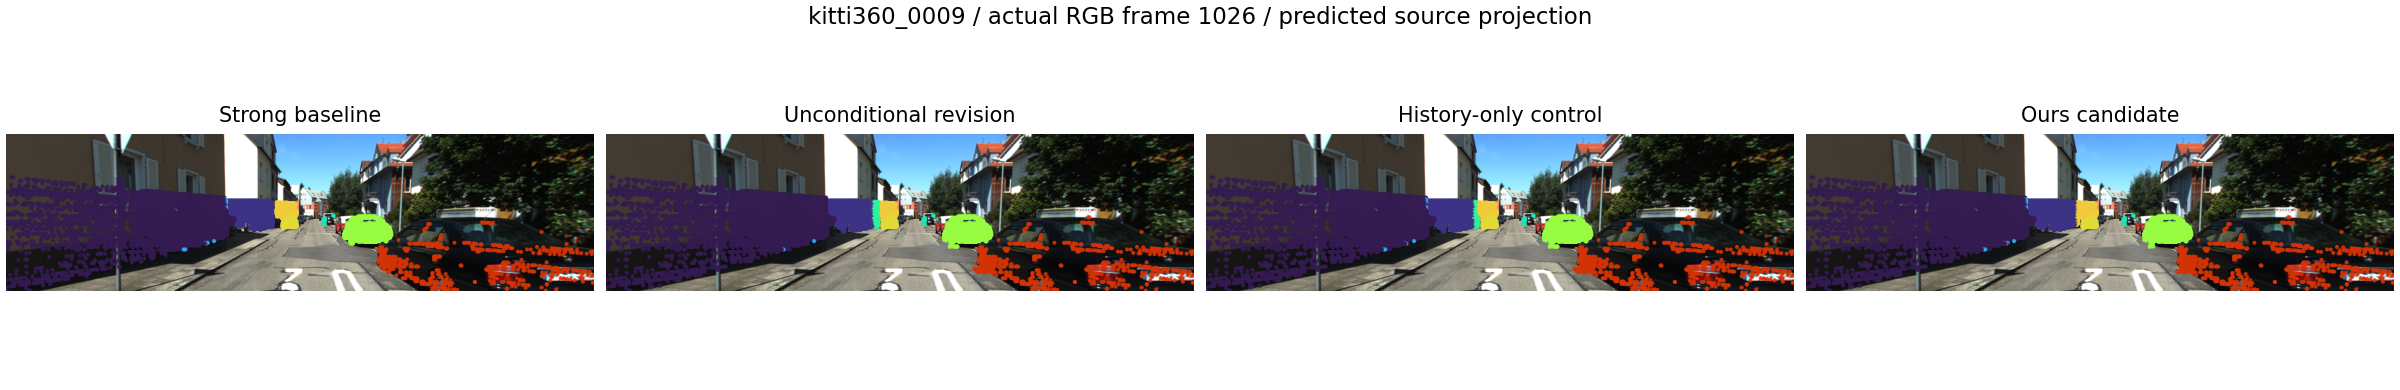
\includegraphics[width=\textwidth]{kitti360_0009_rgb_1026.png}
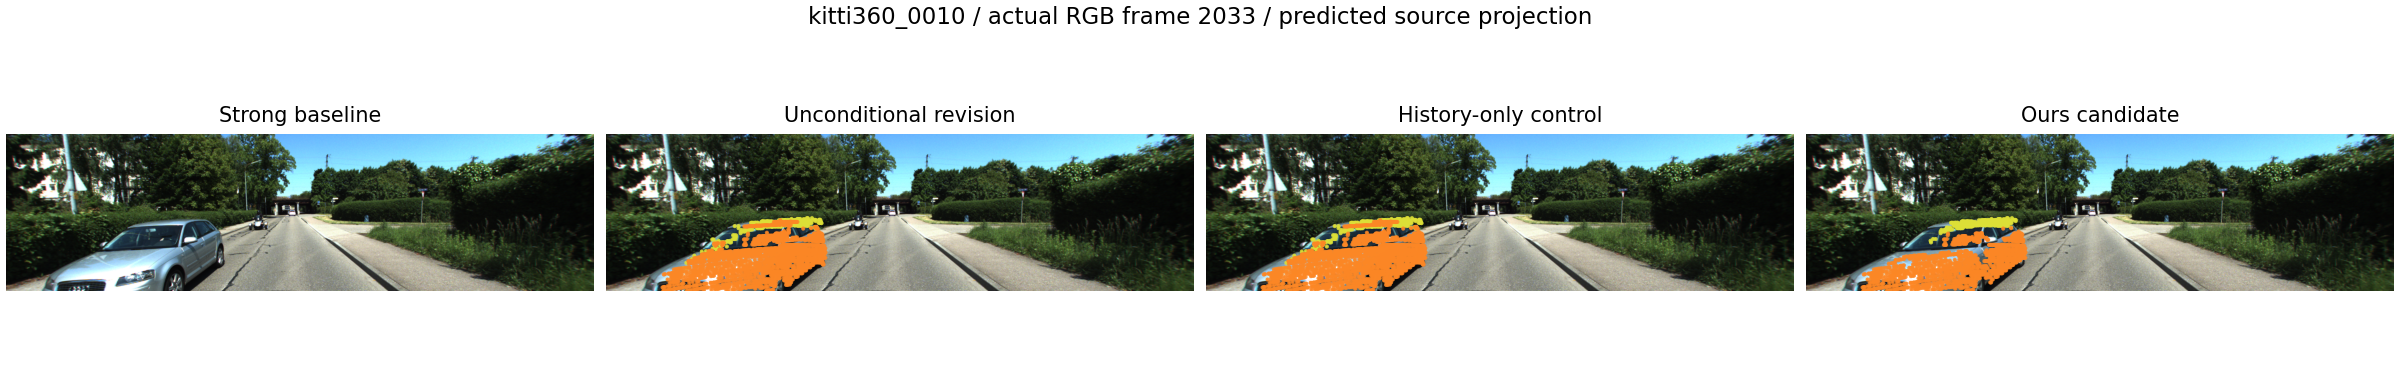
\includegraphics[width=\textwidth]{kitti360_0010_rgb_2033.png}
\captionof{figure}{Actual final sampled RGB frames, with visible measured-source projections from all four maps. Colors are predicted IDs, not GT masks. Display transfer uses 0.05\,m; evaluation uses 0.20\,m. A better-looking car overlay in 0010 does not imply improved car AP, which is identical across methods.}
\end{center}

\begin{center}
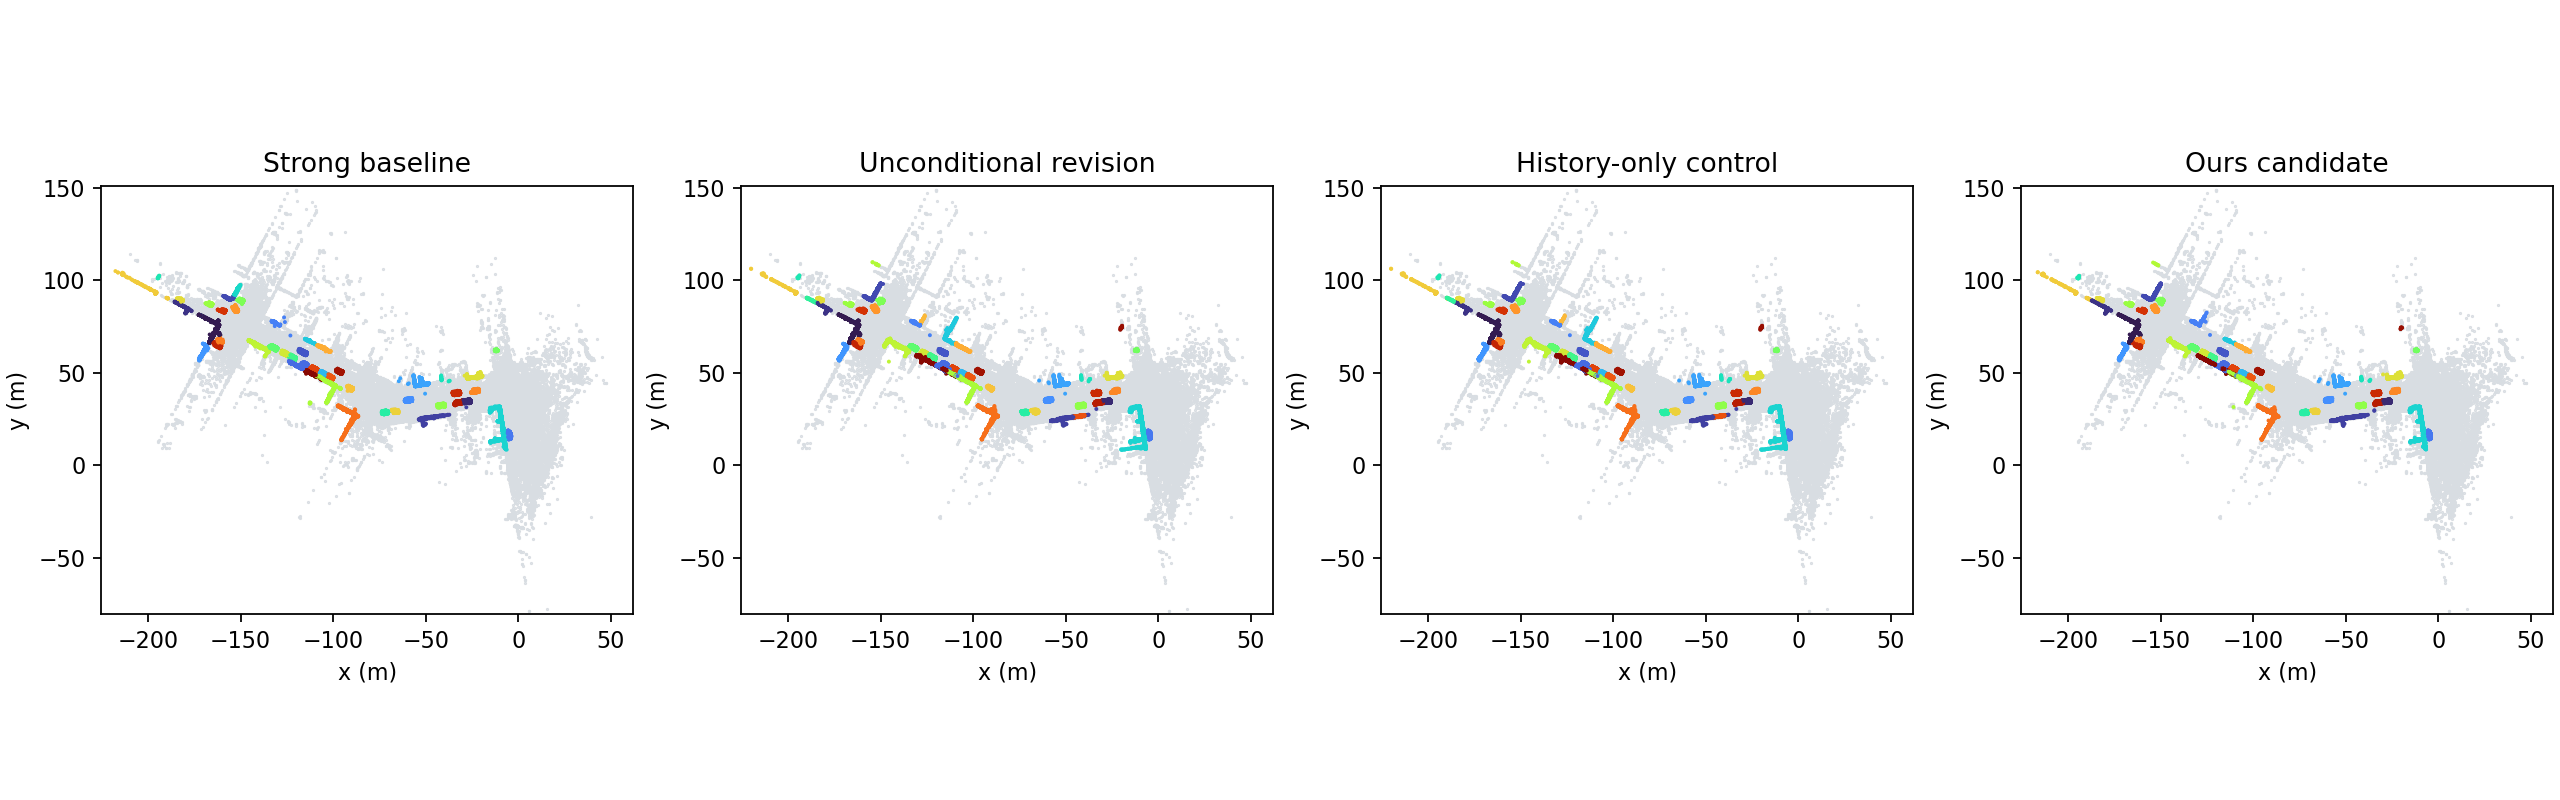
\includegraphics[width=.94\textwidth]{kitti360_0009_maps.png}
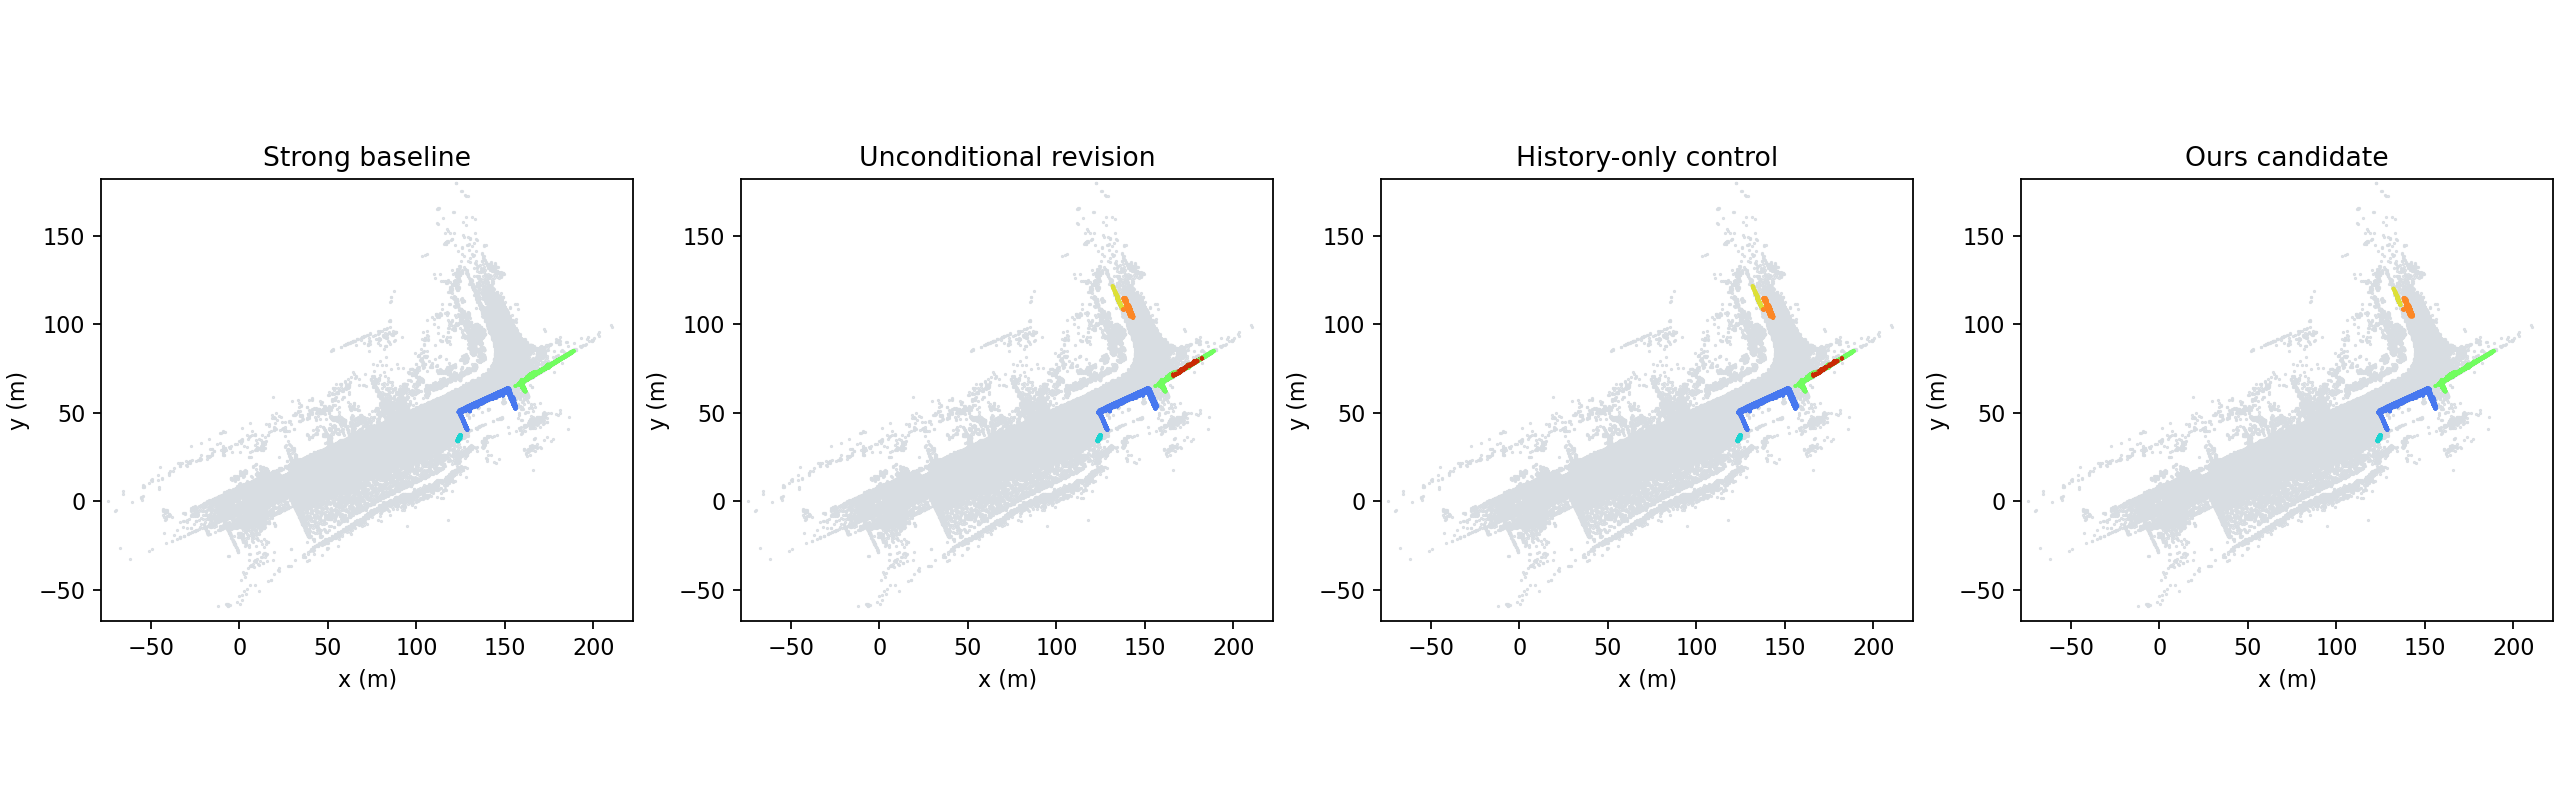
\includegraphics[width=.94\textwidth]{kitti360_0010_maps.png}
\captionof{figure}{Full-window maps with shared measured-source bounds within each row. Gray is measured context; colors are predicted objects. Fixed-stride display subsampling limits context to 60,000 and objects to 40,000 points; scoring uses all exported points.}
\end{center}

\clearpage
\section{Garage Integration}\label{app:robot}
\begin{center}\small\begin{tabular}{lrrr}
\toprule
Method & Points & IDs & Old edits \\
\midrule
Strong baseline & 65,189 & 61 & 0 \\
Unconditional & 1,158,094 & 69 & 11,100 \\
History-only & 1,158,094 & 69 & 0 \\
\textbf{Ours} & 717,816 & 68 & 0 \\
\bottomrule
\end{tabular}
\end{center}
The table uses the same 330 frames and LIVO output. Figure~\ref{fig:robot-current} supplies the exact four-method visual comparison. The retained legacy panels below show baseline, unconditional, \emph{identity-only}, and full \ours. Identity-only is not the history-only control in the table. \ours{} authorizes no historical donor merge here. More points or IDs do not establish higher accuracy.

\begin{center}
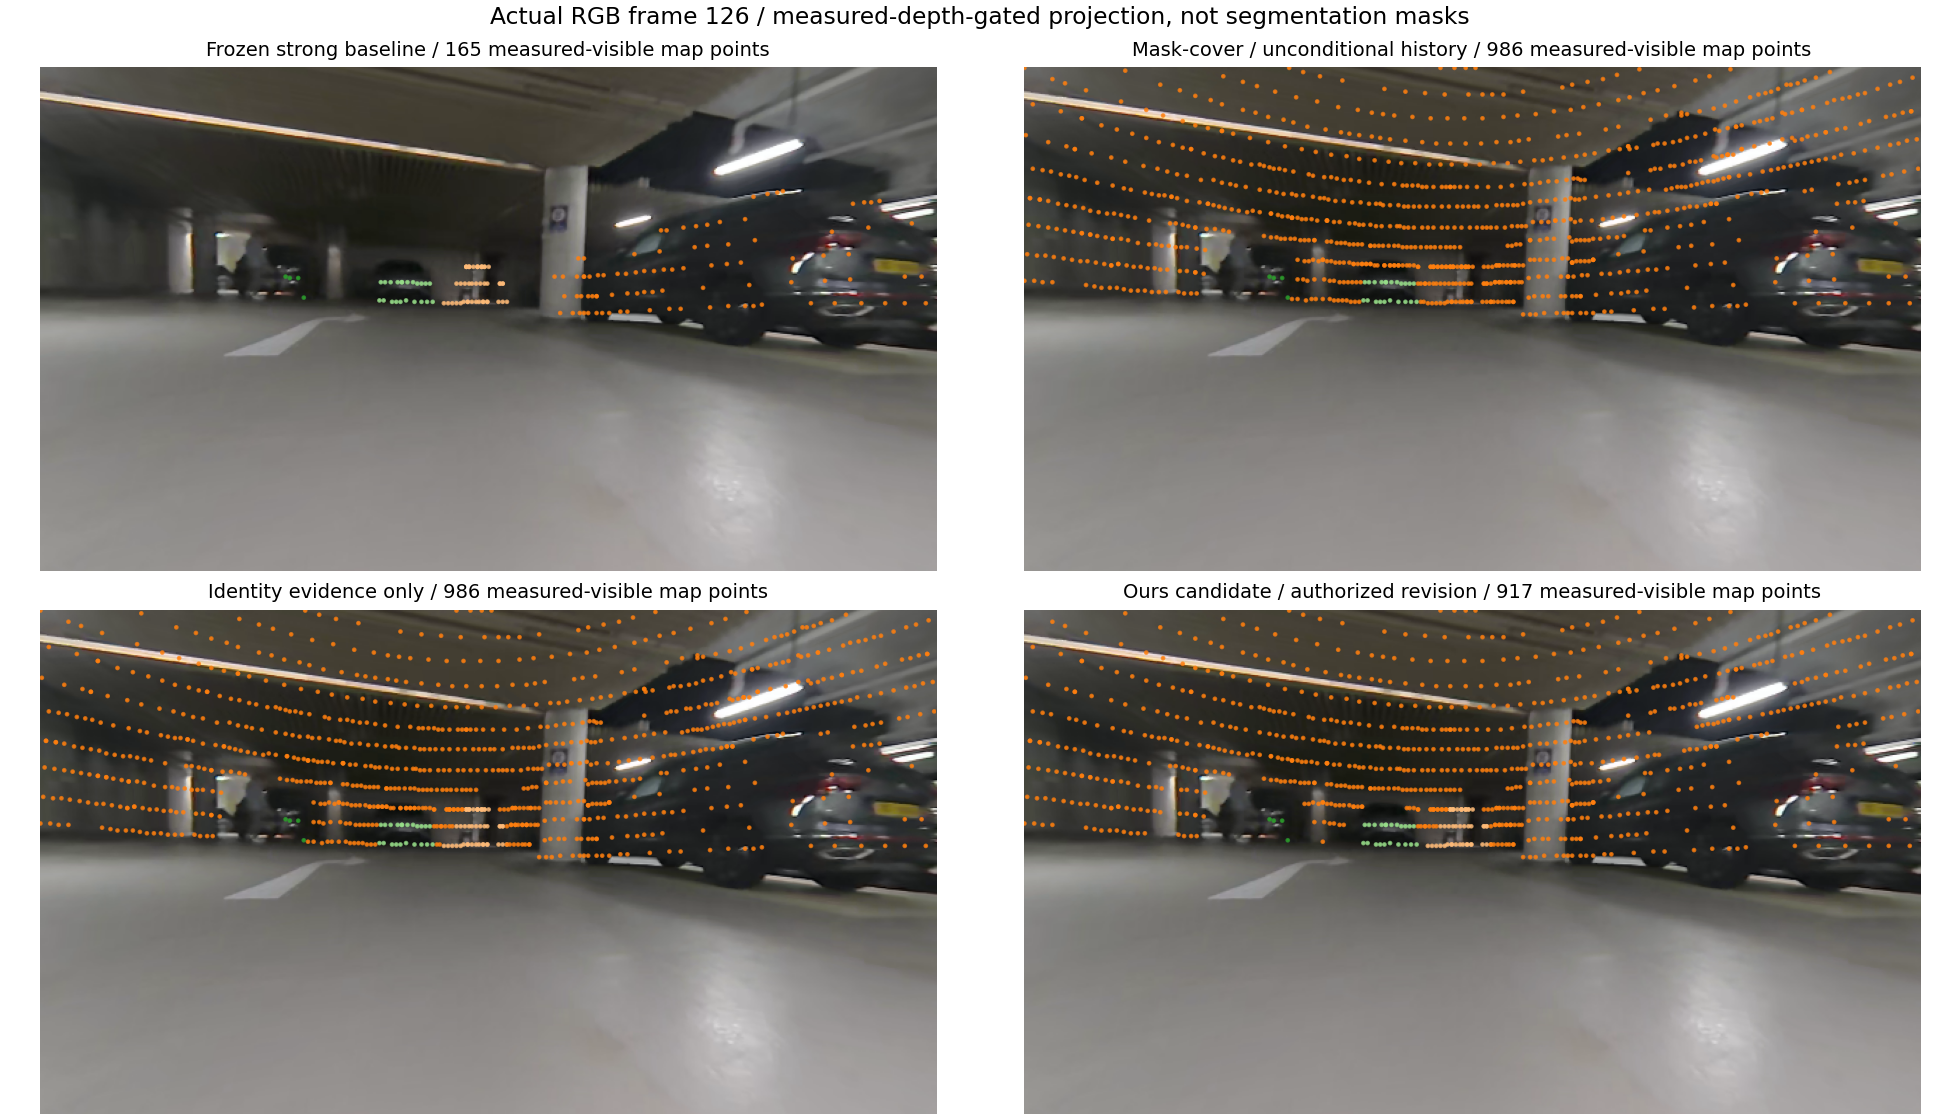
\includegraphics[width=.74\textwidth]{robot_frame_000126.png}
\captionof{figure}{Actual garage frame and measured projection diagnostic. A qualitative integration example without independent contours or identity GT.}
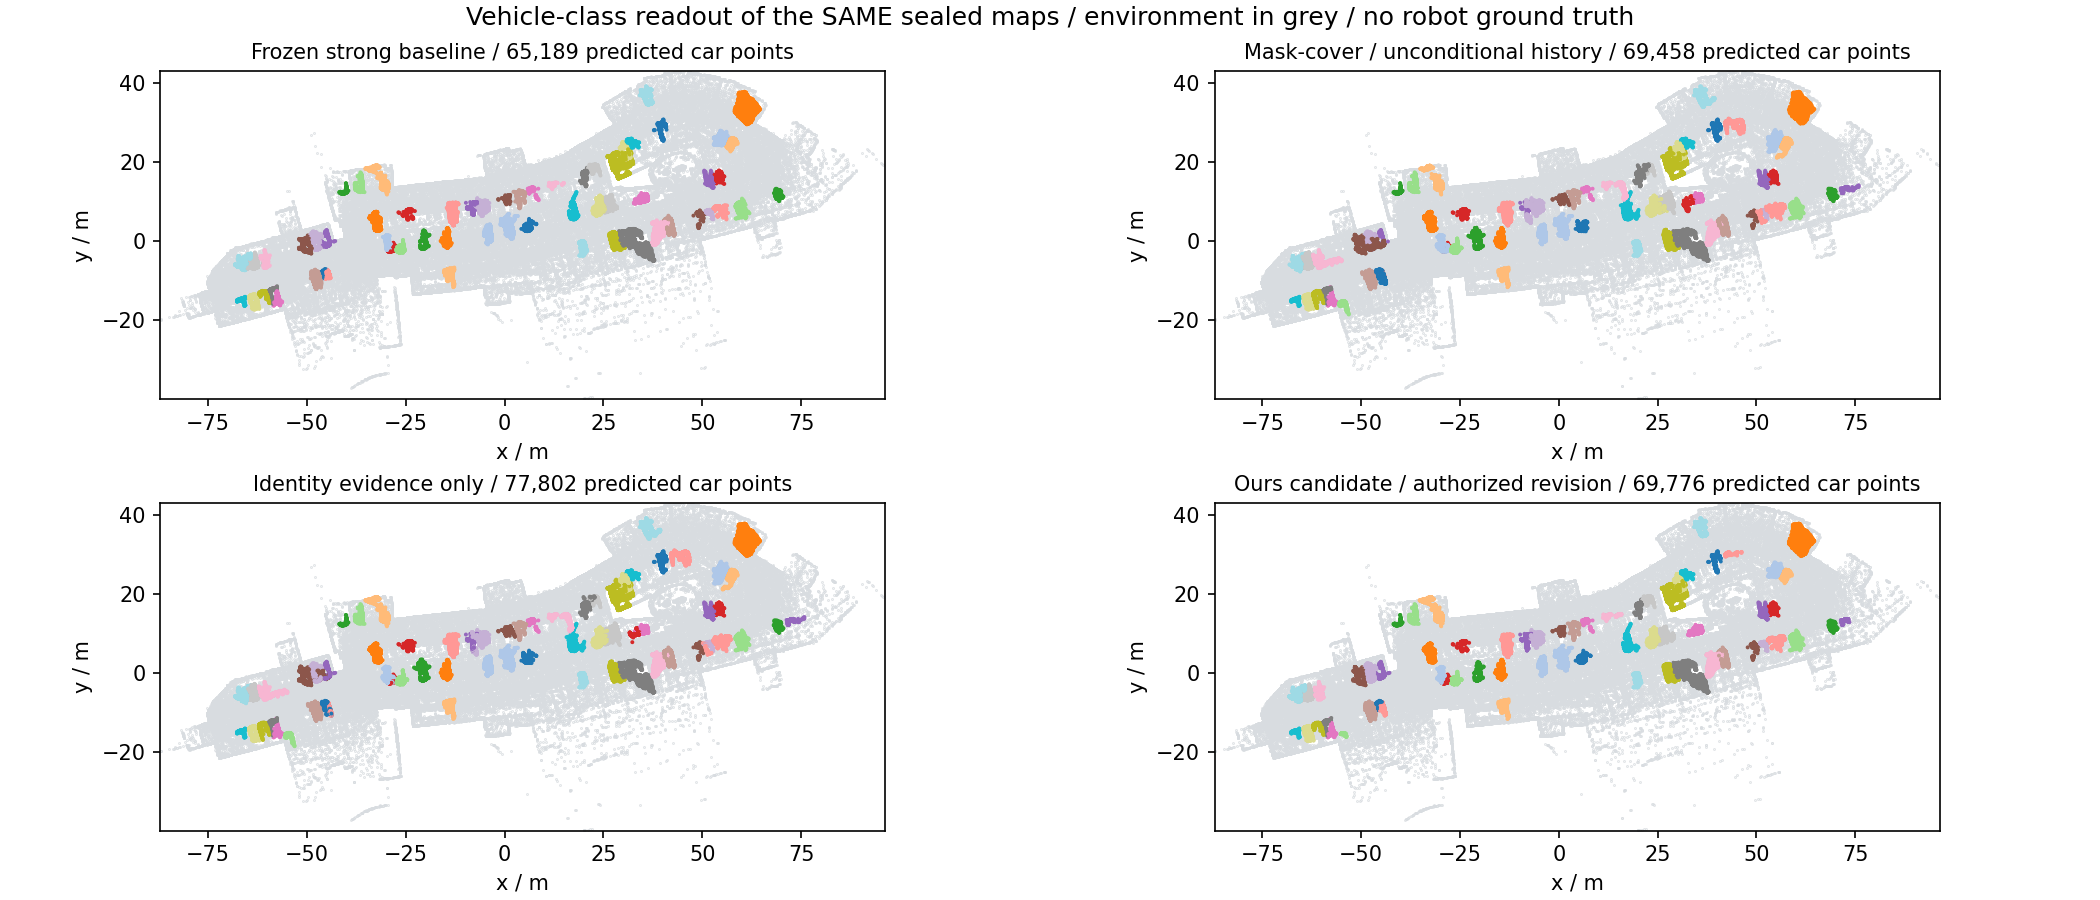
\includegraphics[width=.74\textwidth]{robot_vehicles.png}
\captionof{figure}{Actual garage vehicle-map comparison. Archive visibility is offline; no claim of causal online semantics, S100 runtime, or semantic-accuracy improvement follows.}
\end{center}

\subsection{Evaluation scope}
The garage comparison demonstrates that the same revision kernels operate on LIVO outputs. Independent vehicle contours and cross-frame identities are unavailable, so semantic accuracy cannot be measured here. Public-data comparisons, including the completed spatial extension, appear in Appendix~\ref{app:extension}.
\clearpage
\subsection{Current table-aligned garage comparison}
The following figure uses the four sealed maps in the garage table and the same recorded frame 126. History-only uses the authorized old-label prefix and unconditional new geometry; it is not the identity-only control in the retained panels.

\begin{center}
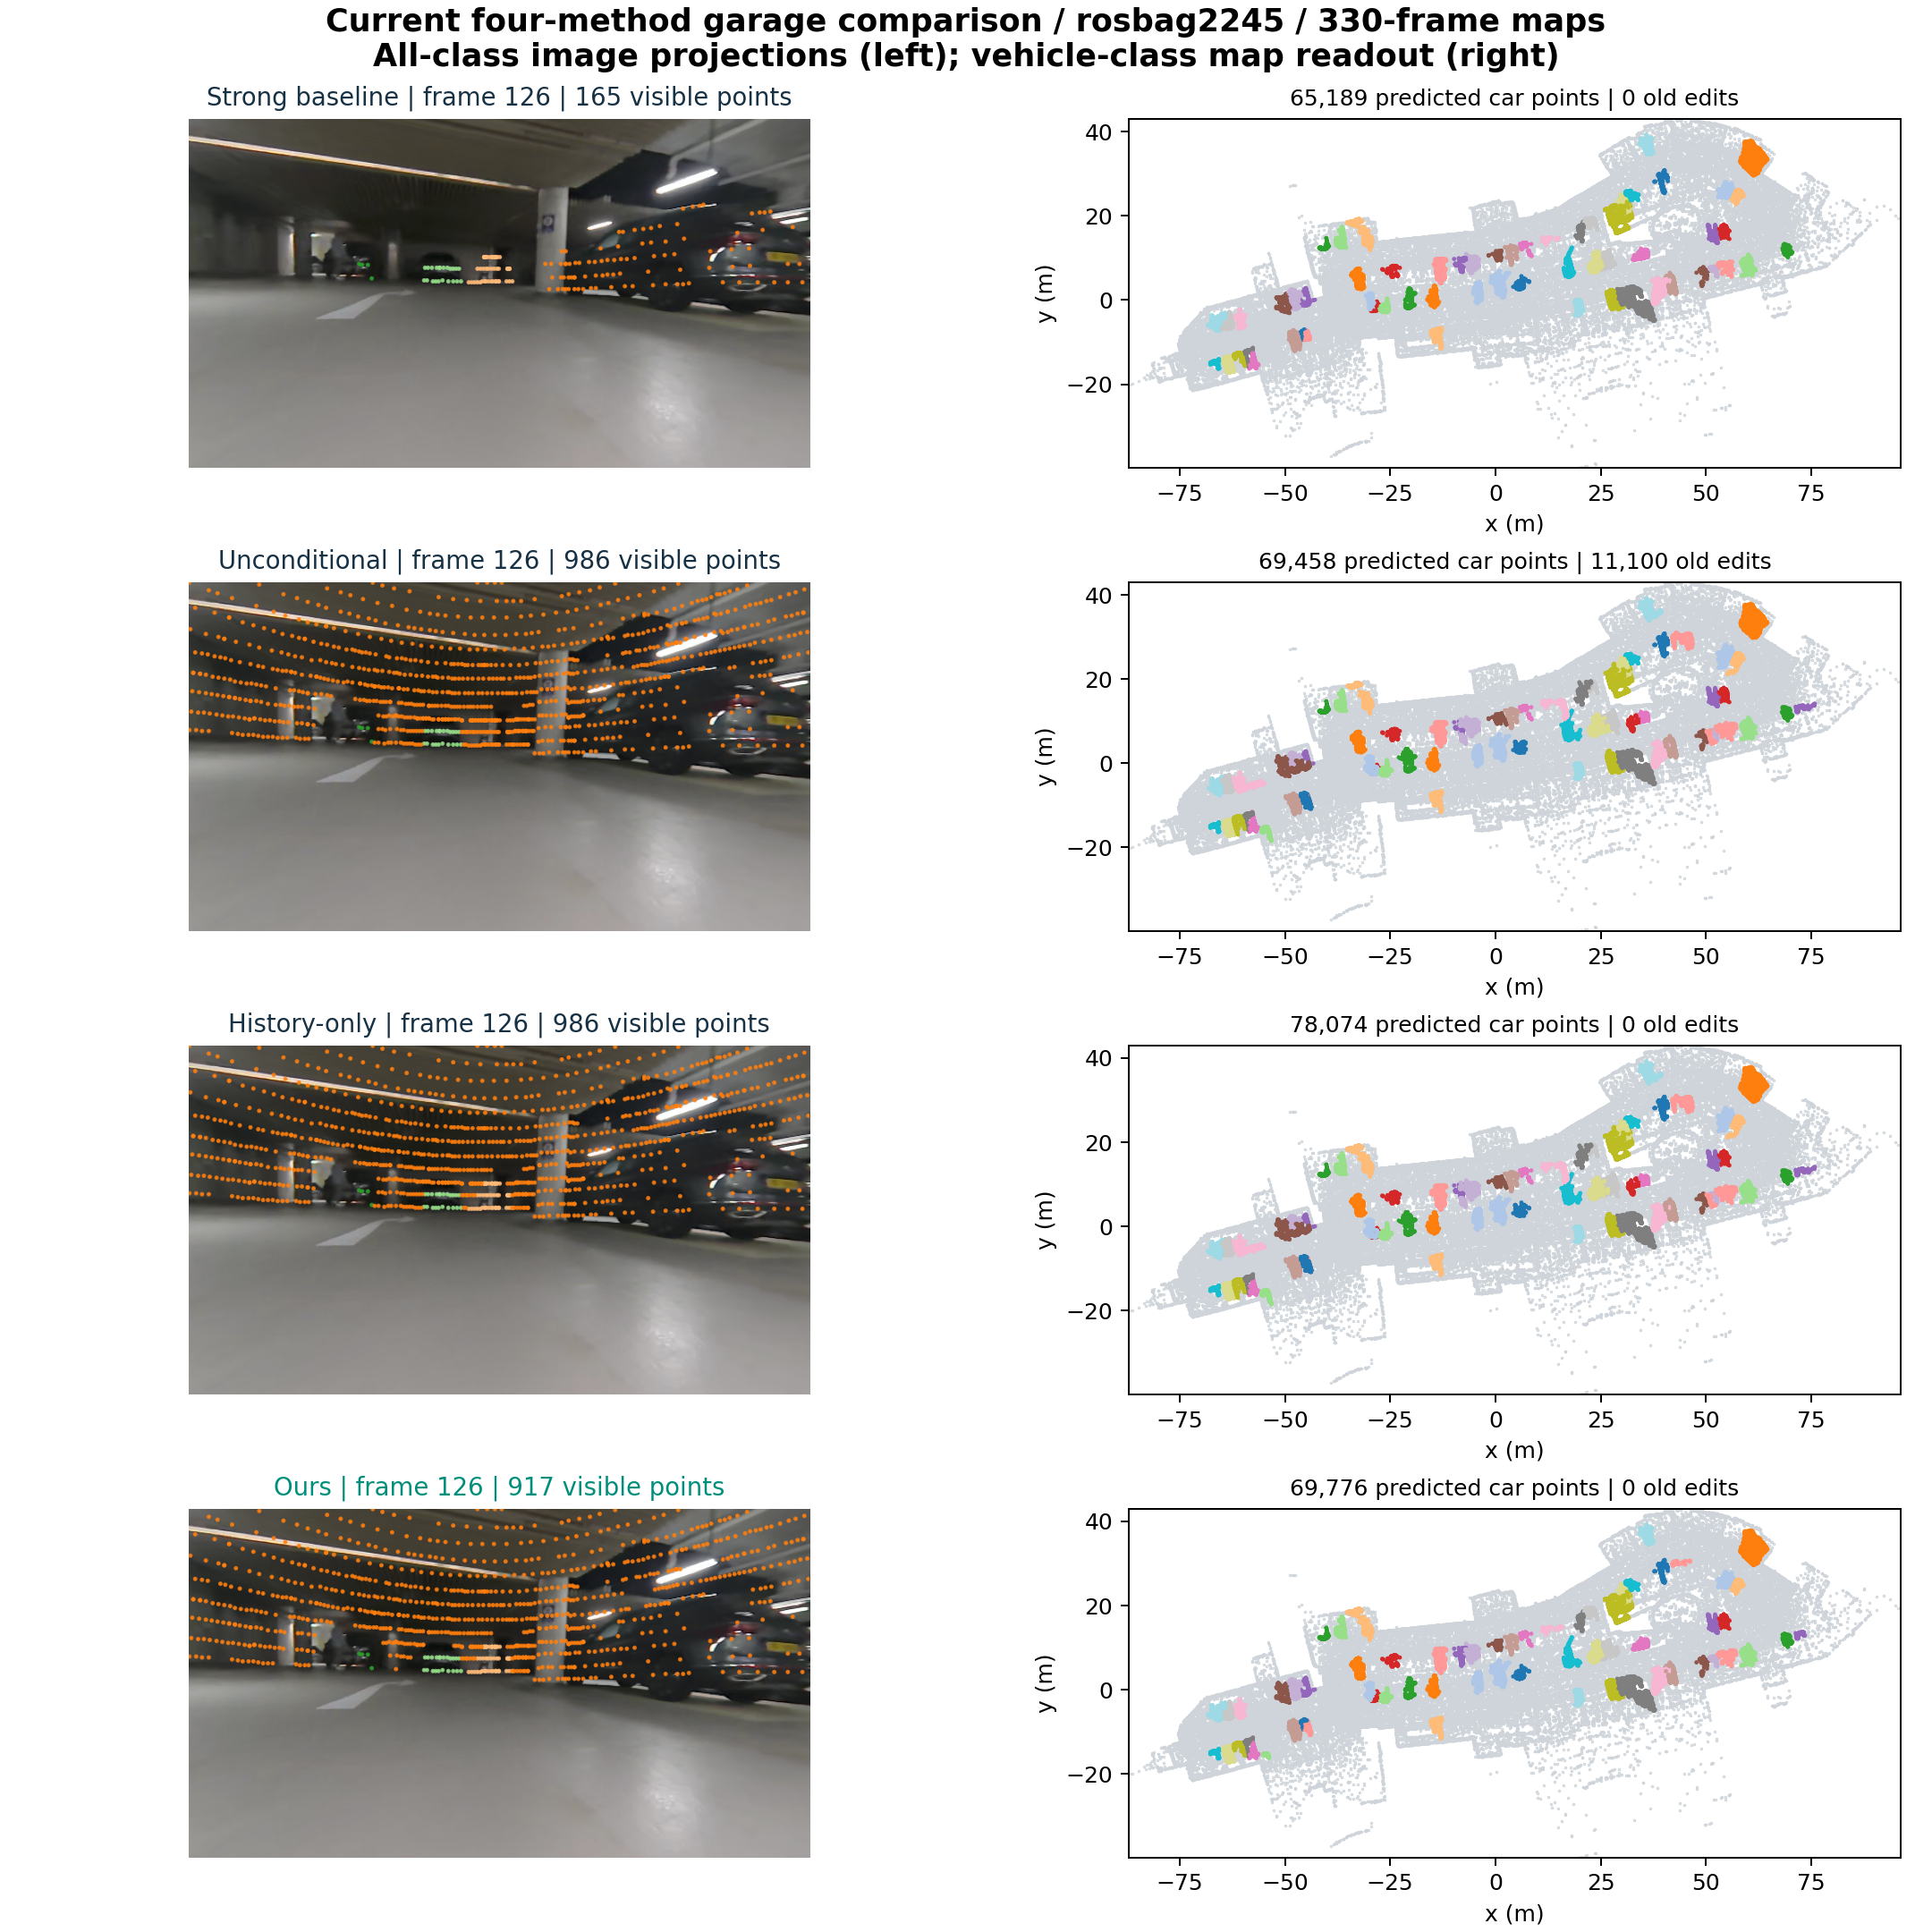
\includegraphics[width=.97\textwidth]{robot_current_four.png}
\captionof{figure}{Current baseline, unconditional, history-only, and Ours on the same 330-frame garage map. Left: actual RGB with all-class, measured-depth-gated point projections. Right: predicted vehicle-class points on shared map bounds; gray context is deterministically subsampled to 60,000 points, while vehicle points are unthinned. The repeated identity palette does not establish cross-method physical correspondence. Archive visibility is offline. Vehicle-point counts are 65,189 / 69,458 / 78,074 / 69,776; greater support is not an accuracy measurement.}
\label{fig:robot-current}
\end{center}

\section{Controlled Output Interventions}\label{app:causal}
The five interventions per prospective window were specified after the primary results were inspected and before intervention scoring. They hold weights, thresholds, proposals, and original predictions fixed. Their effects are conditional on those decisions.

\paragraph{Historical-label controls.}
``Ours new'' copies Ours appended sources, coordinates, labels, and ranking metadata. Replacing only the historical-label prefix with either baseline or unconditional labels measures the effect of old assignments at fixed new geometry. Old-point coordinates and ordering are unchanged.

\paragraph{New-point controls.}
``Witness'' keeps directly mask-supported parent additions with their parent labels, paired with either preserved or authorized history. ``Nearest'' fixes Ours history and assigns supported additions to the unique nearest seed identity without the second seed-frame requirement on new points. Historical authorization, including its local check, remains fixed. All controls share the Ours classification metadata and postprocessing.

\begin{center}\small
\begin{tabular}{@{}lrrr@{}}
\toprule
Export intervention & 0009 & 0010 & Mean \\
\midrule
Unconditional old IDs + Ours new & 23.253 & 11.420 & 17.337 \\
Preserved old IDs + Ours new & 23.166 & 14.198 & 18.682 \\
Preserved old IDs + witness & 23.089 & 12.809 & 17.949 \\
Authorized old IDs + witness & 23.230 & 12.809 & 18.019 \\
Authorized old IDs + nearest & 23.327 & 14.198 & 18.762 \\
\textbf{Ours (fixed)} & 23.327 & 14.198 & 18.762 \\
\bottomrule
\end{tabular}

\captionof{table}{All controlled output interventions, AP50:90 in percent. Only the operations specified above vary.}
\end{center}

For 0009, the nearest-seed control retains 35 sources rejected by Ours and differs at five reference positions, yet AP is equal. For 0010, its source set, labels, and reference predictions are identical to Ours. The witness-history versus witness-preservation contrast is +0.141 / +0.000 AP points in 0009/0010. These paired effects depend on which additions are held fixed and need not sum to the total baseline-to-Ours change.

\subsection{Interpreting historical edits}
Each baseline predicted ID is matched to the same-class canonical reference instance with maximum confidence-weighted intersection; ties use the lower reference ID. Multiple fragments may match the same instance, and IDs without same-class overlap remain unmapped. This correspondence is then held fixed across variants. Each reference point retains its nearest baseline source within 0.20\,m, and only the historical label at that source changes.

For mapped endpoints, wrong-to-correct transitions are corrections, correct-to-wrong transitions are damage, and correct-to-correct transitions consolidate fragments of the same reference object. Wrong-to-wrong transitions remain unresolved. Missing endpoint correspondences and void reference points are reported separately. Counts other than ``Old edits'' are confidence-weighted reference mass, rather than source-point accuracy.

\begin{center}\footnotesize
\begin{tabular}{@{}llrrrrrr@{}}
\toprule
Window & Method & Old edits & Correction & Damage & Consolidation & Unresolved & Unknown \\
\midrule
0009 & Unconditional & 26,788 & 101.1 & 1072.9 & 10848.0 & 7152.8 & 3348.2 \\
0009 & \textbf{Ours} & 12,855 & 0.0 & 0.0 & 10671.7 & 2.7 & 0.0 \\
0010 & Unconditional & 3,427 & 0.0 & 0.0 & 0.0 & 0.0 & 3552.2 \\
0010 & \textbf{Ours} & 0 & 0.0 & 0.0 & 0.0 & 0.0 & 0.0 \\
\bottomrule
\end{tabular}

\captionof{table}{Historical outcomes under a fixed baseline-to-reference correspondence. Unknown endpoints are excluded from correct/incorrect categories.}
\end{center}

The authorized 0009 transitions are $27\!\to\!17$ (8,745 sources, building 2168) and $36\!\to\!48$ (4,110 sources, building 2486). Both consolidate fragments of the same object; 2.736 reference mass remains wrongly assigned. The unconditional 0010 transition targets ID 6, which is absent from the baseline correspondence, leaving 3,552.226 reference mass unknown in this diagnostic. Its effect on AP is measured by the fixed-new-geometry intervention in Table~\ref{tab:causal}.

\section{Runtime and External Comparison}\label{app:runtime}
\subsection{Revision runtime}
On an AMD Ryzen 9 9950X, cached graph assignment takes 117.66\,ms for 0009 and 17.33\,ms for 0010. The graph timer includes both native multi-source distance searches and the certificate calculation. The pair timer evaluates merge decisions from cached per-view evidence. Model inference, projection, proposal construction, loading, and export are excluded. These are single CPU runs rather than end-to-end latency estimates.

\begin{center}\small
\begin{tabular}{@{}lrrrrrr@{}}
\toprule
Window & Nodes & Edges & Seeds & Graph (ms) & Pairs (ms) & Prior prep. (s) \\
\midrule
0009 & 42,955 & 457,332 & 61,886 & 117.66 & 0.180 & 5.201 \\
0010 & 15,091 & 129,426 & 11,665 & 17.33 & 0.001 & 2.323 \\
\bottomrule
\end{tabular}

\captionof{table}{Revision input sizes and component timings. Edges are directed. Prior preparation was measured in a separate run and is not added to the replay timers.}
\end{center}

The replay driver's peak resident memory is 198.4\,MiB across the two cached runs. Map export takes 0.286--0.290\,s for 0009 and 0.088--0.089\,s for 0010. Native distances and certificate arrays reproduce the archived results exactly. The geometry weights were fitted on exposed 0000/0002 data; neither the replay nor the extension refits them.

\subsection{MaskClustering core adaptation}\label{app:external}
We run the official MaskClustering graph construction, iterative view-consensus clustering, and postprocessing code through a CPU adapter. Six upstream files are pinned; only device substitutions and an unused backprojection import are changed. Inputs are disjoint highest-score SAM3 query supports on the same measured sources, using the causal visibility cache. Query scores provide the building/car readout. This replaces the native CropFormer~\cite{cropformer}/OpenCLIP~\cite{openclip} frontend and also differs from the internal backbone's semantic readout.

We retain the upstream ScanNet defaults: visible and undersegmentation ratios 0.3, consensus 0.9, contained-mask ratio 0.8, point-filter ratio 0.5, DBSCAN radius 0.1\,m with four minimum points, two supporting masks, and overlap merge ratio 0.8. Empty graphs export no clusters. Source ties use stable object order in the nearest-map readout.

\begin{center}\small
\begin{tabular}{@{}lrrr@{}}
\toprule
Window & Primary AP & Canonical AP & Uniform-score AP \\
\midrule
0009 & 0.0071 & 0.0082 & 0.1664 \\
0010 & 0.0000 & 0.0000 & 0.0000 \\
\bottomrule
\end{tabular}

\captionof{table}{MaskClustering core adaptation on the prospective windows. AP is reported in percent; the four-window extension is included in Table~\ref{tab:results}b.}
\end{center}

The adapter yields 2,542 / 662 intermediate clusters and 98 / 23 final objects on 0009/0010. Fragmentation is severe and AP is low. Because the inputs and readout have changed and indoor defaults are retained, this comparison diagnoses the adaptation; it cannot establish superiority over the native MaskClustering pipeline.

\clearpage
\section{V1: Fixed-Identity Geometry Study}\label{app:v1}
This appendix preserves the earlier algorithm and its evidence. Every occurrence of ``Ours'' embedded in a retained V1 figure denotes V1 only; the current method is identified as \ours{} in the new main result and outdoor appendices. The versions do not share an evaluation protocol.

\subsection{Depth-conditioned support, refutation, and deletion}
For source point $p$ assigned to object $o$, V1 projects into frames with an assigned observation. It requires positive camera depth $z>0.2$\,m and a finite positive measured depth $D$ satisfying $|z-D|\leq0.05\,\mathrm m+0.01D$. An eligible projection supports $o$ inside its eroded mask union, or refutes $o$ inside another known mask outside the dilated union. The erosion/dilation radius is two pixels. Unknown pixels, occlusions, and uncertain boundaries abstain; overlapping masks contribute at most one vote per point/frame. With support $S_o(p)$ and refutation $R_o(p)$ accumulated over eligible frames, V1 deletes exactly when
\begin{equation}
R_o(p)\geq1\quad\land\quad R_o(p)\geq2S_o(p).
\label{eq:v1-rule}
\end{equation}
For nonzero evidence this is equivalent to support share $S/(S+R)\leq1/3$; zero-evidence points remain. It cannot append surfaces, create objects, split mergers, or revise identity. Statistical outlier removal (SOR)~\cite{sor} uses each object's mean 20-neighbor distance with a mean-plus-two-standard-deviations cutoff. These are separate point-selection mechanisms.

\subsection{Configuration selection}
Replica~\cite{replica} office\_0/office\_1 and SceneNN 014/015 were exposed development data. The pilot primary required three refutations. Before processing the four new SceneNN scenes, the existing one-refutation arm was selected empirically: its dataset-mean gains were +2.018 and +1.034 points, versus +2.002 and +0.656 for three refutations. Only the minimum count changed; the depth gate, boundaries, and refutation/support ratio remained fixed. This did not make the original two-point-per-dataset pilot requirement pass. V1 also remained below SOR in the subsequent four-scene mean. No configuration was selected after those new-scene scores.

\begin{center}\small
\begin{tabular}{lrrrrr}
\toprule
Scene & Baseline & SOR & Three-frame & No depth (3) & V1 (1) \\
\midrule
office\_0 & 30.923 & 31.249 & 34.017 & 33.589 & 34.078 \\
office\_1 & 47.019 & 47.752 & 47.928 & 45.289 & 47.900 \\
SN 014 & 15.868 & 16.452 & 17.133 & 17.068 & 17.824 \\
SN 015 & 14.408 & 14.669 & 14.454 & 14.422 & 14.519 \\
\bottomrule
\end{tabular}

\captionof{table}{V1 development PQ, kept separate from both SceneNN new-scene and current KITTI-360 results. ``No depth (3)'' uses three refutations, unlike the one-refutation no-depth control in the SceneNN main table.}
\end{center}

\begin{minipage}[t]{.49\textwidth}\vspace{0pt}\centering\small
\begin{tabular}{lrr}
\toprule
Contrast & $\Delta$ PQ & Wins/losses \\
\midrule
V1 -- baseline & +0.841 & 4/0 \\
V1 -- SOR & -0.050 & 3/1 \\
V1 -- no depth & +0.454 & 2/2 \\
V1 -- three-frame & +0.136 & 4/0 \\
V1 locked -- baseline & +1.095 & 4/0 \\
SOR locked -- baseline & -0.287 & 2/2 \\
\bottomrule
\end{tabular}

\captionof{table}{V1 paired contrasts on four SceneNN scenes. Locked assignment is a diagnostic, not the primary metric.}
\end{minipage}\hfill
\begin{minipage}[t]{.48\textwidth}\vspace{0pt}\centering\small
\begin{tabular}{lrrrr}
\toprule
Scene & Objects & Points & Evidence (s) & Job (s) \\
\midrule
052 & 89 & 48,231 & 0.286 & 1.583 \\
054 & 121 & 70,796 & 0.458 & 1.949 \\
057 & 31 & 38,377 & 0.262 & 1.236 \\
061 & 12 & 60,913 & 0.391 & 1.836 \\
\bottomrule
\end{tabular}

\captionof{table}{V1 archived CPU timers and map scale. Evidence jointly times gated and ungated voting; job includes loading, SOR, cleanup variants and exports. Neither is isolated V1 latency or current-method speed.}
\end{minipage}

\subsection{Matched-set and assignment interpretation}
V1's 66 SceneNN matches are unchanged. At GT 136313 in scene 057, V1 gives IoU 0.496947 while SOR reaches 0.535340. V1 removes 92 source points and SOR removes 97: deletion count alone does not explain the ranking. Of 410 excess baseline reference voxels, 304 have owners with support but no refutation. Under locked baseline source ownership, V1 instead reaches IoU 0.501247; ordinary reassignment adds five correct and 17 excess voxels. Nearest-source reassignment therefore changes the measured effect of point deletion.


\clearpage
\section{V1 Architecture and Visibility Evidence}\label{app:v1-architecture}
The diagram below preserves the complete fixed-identity architecture and its evidence flow. It complements the current authorization architecture in Figure~\ref{fig:architecture}; the two diagrams describe different update operations.
\begin{center}
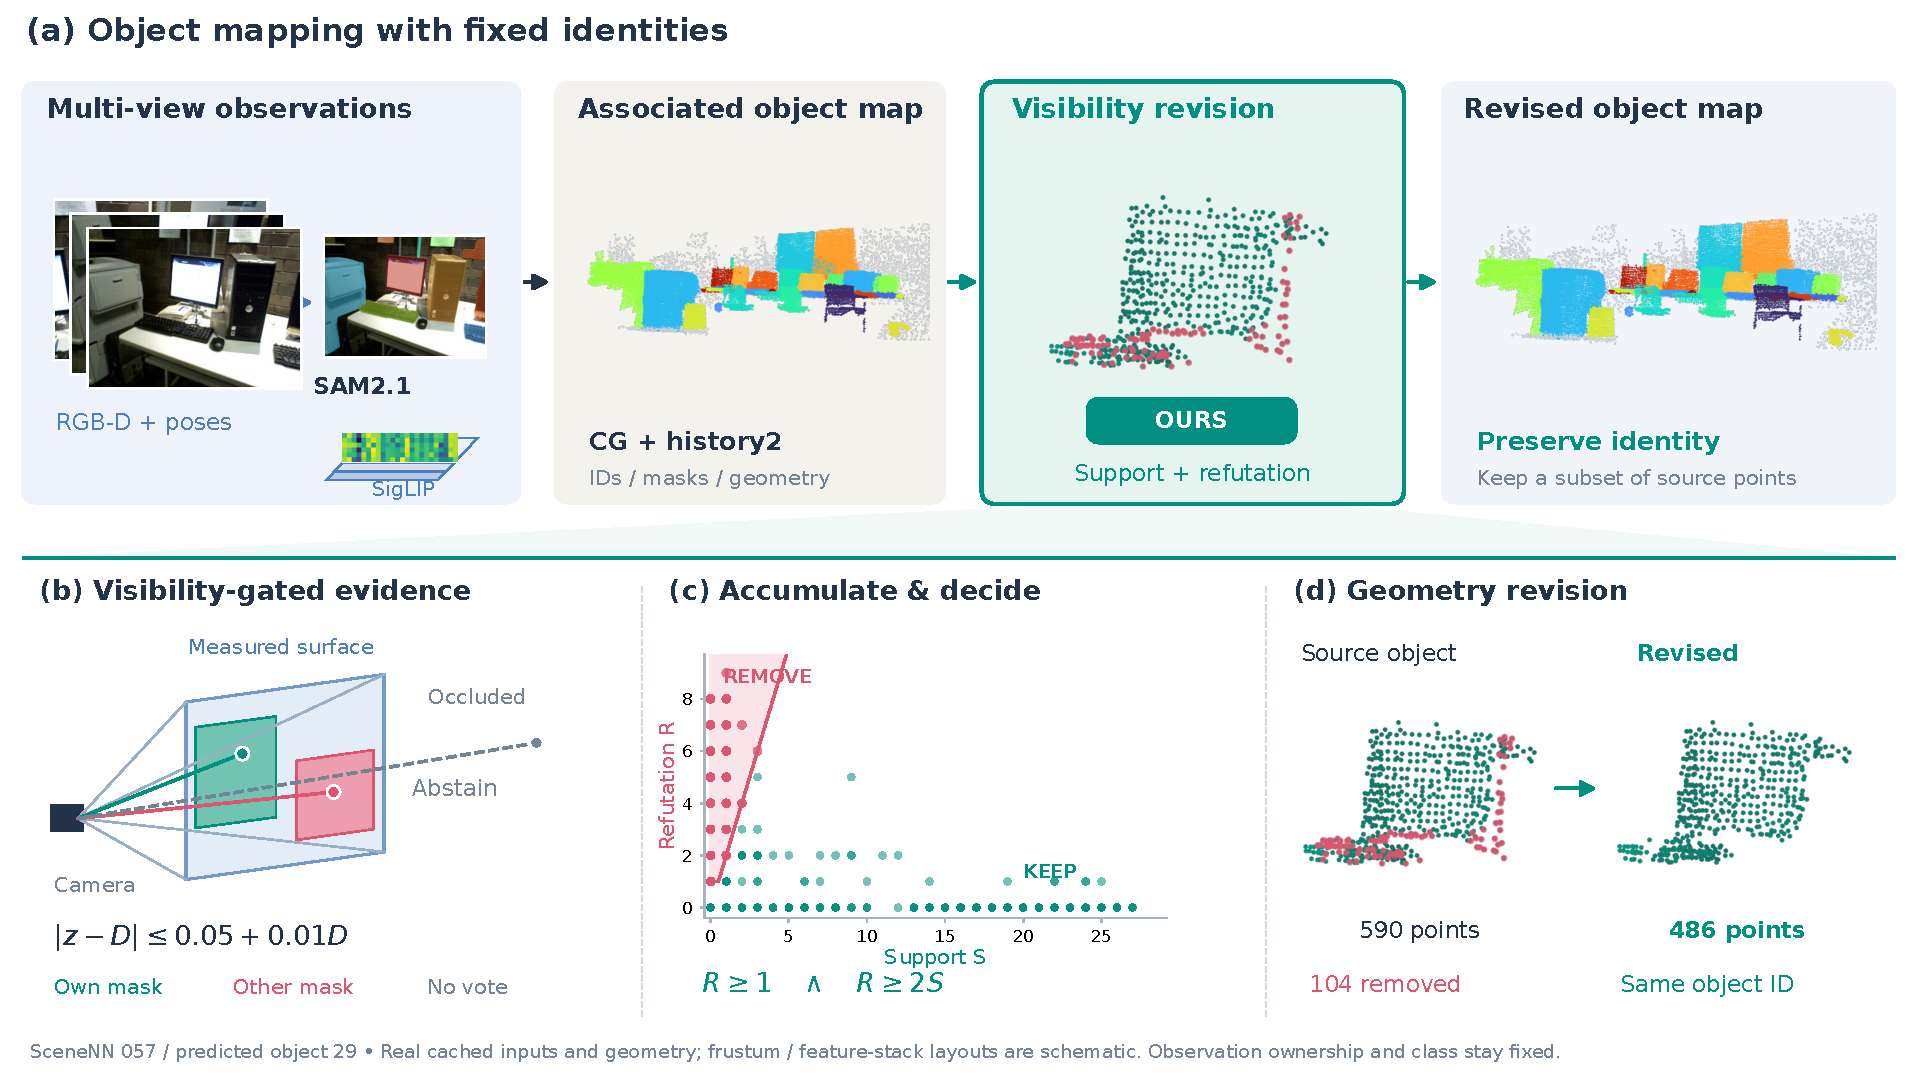
\includegraphics[width=\textwidth]{method_architecture.pdf}
\captionof{figure}{Retained V1 architecture with actual SceneNN observations, cached descriptors, source-point evidence, and revised object geometry. The embedded ``OURS'' block denotes V1. It retains a subset of existing source points while keeping identities, observation ownership, and semantic classes fixed. View frustums and the feature-stack layout are schematic.}
\label{fig:v1-architecture}
\end{center}
\subsection{Reading the two architectures together}
V1 asks whether a point already assigned to an object should remain in that object. Depth gating defines eligible observations; support and refutation determine deletion. It does not grant permission to change the historical identity of a point or append missing measurements.

The current method adds historical relabeling and measured-surface admission to the available updates. Figure~\ref{fig:architecture} shows this extension; the pose source remains fixed in both studies.

\clearpage
\section{Retained Indoor Image and Object Evidence}
\begin{center}
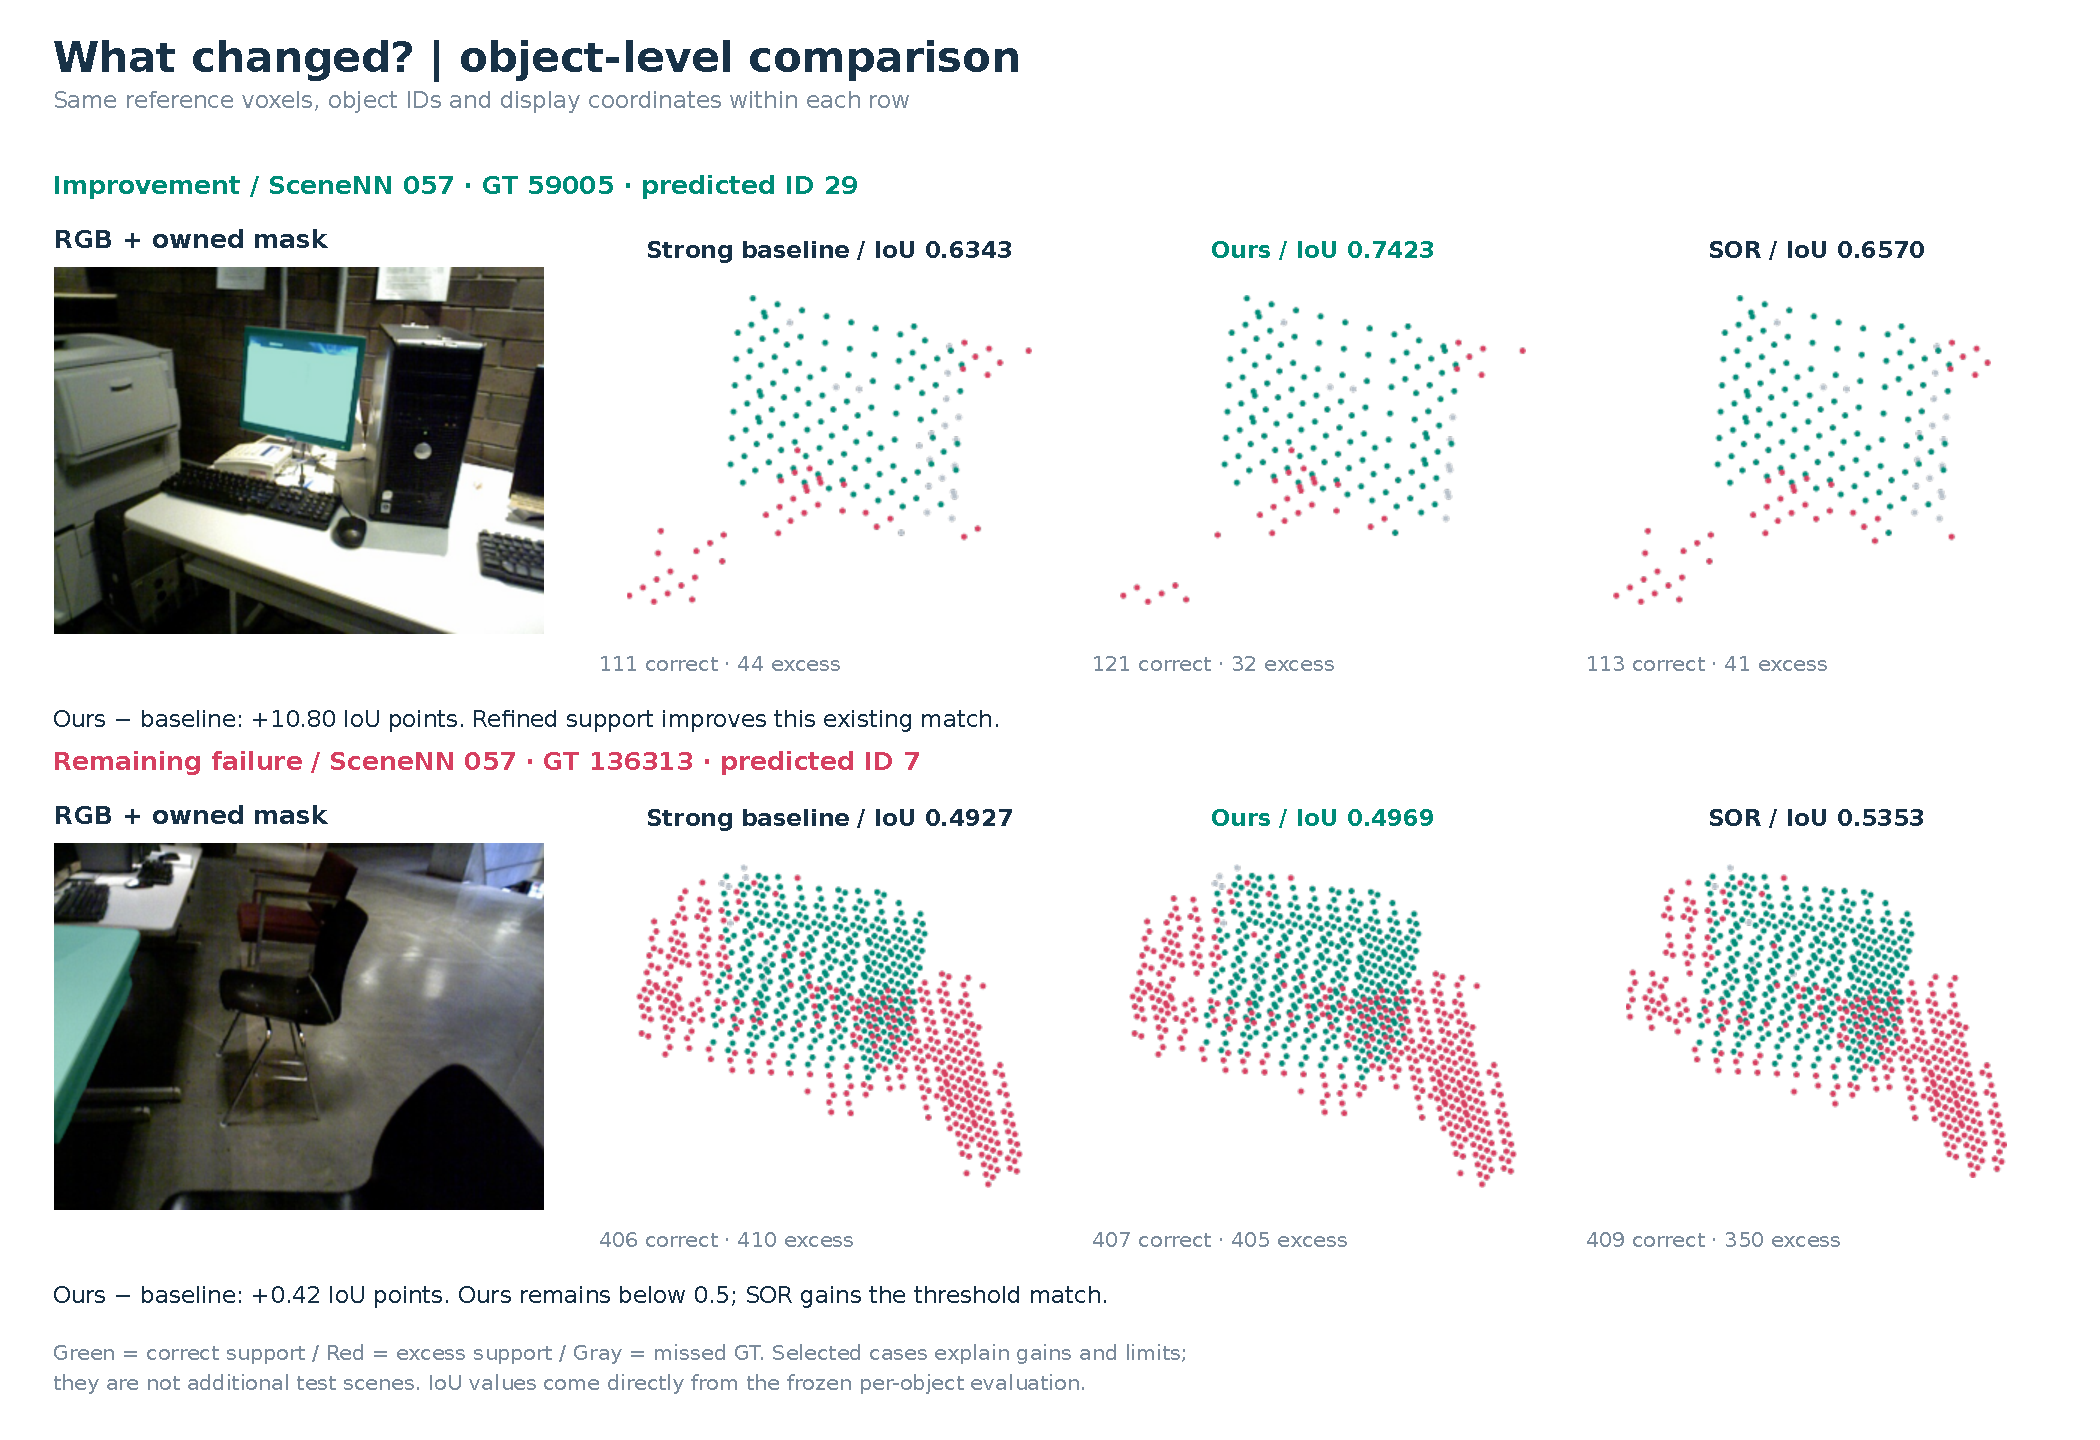
\includegraphics[width=\textwidth]{object_comparison_real.pdf}
\captionof{figure}{Actual SceneNN 057 observations and same-object geometry from V1. Embedded ``Ours'' labels mean V1. The monitor improves from IoU 0.6343 to 0.7423; the second object remains below 0.5 while SOR crosses it. These were post-evaluation explanatory selections, not random samples.}
\end{center}
These indoor images use supplied RGB-D poses and the SAM2.1/SigLIP branch. The following two pages retain each scene at full width so that RGB, masks, colored geometry, and predicted object boundaries can be inspected separately.

\clearpage
\section{SceneNN 057: Observations and V1 Map}
\begin{center}
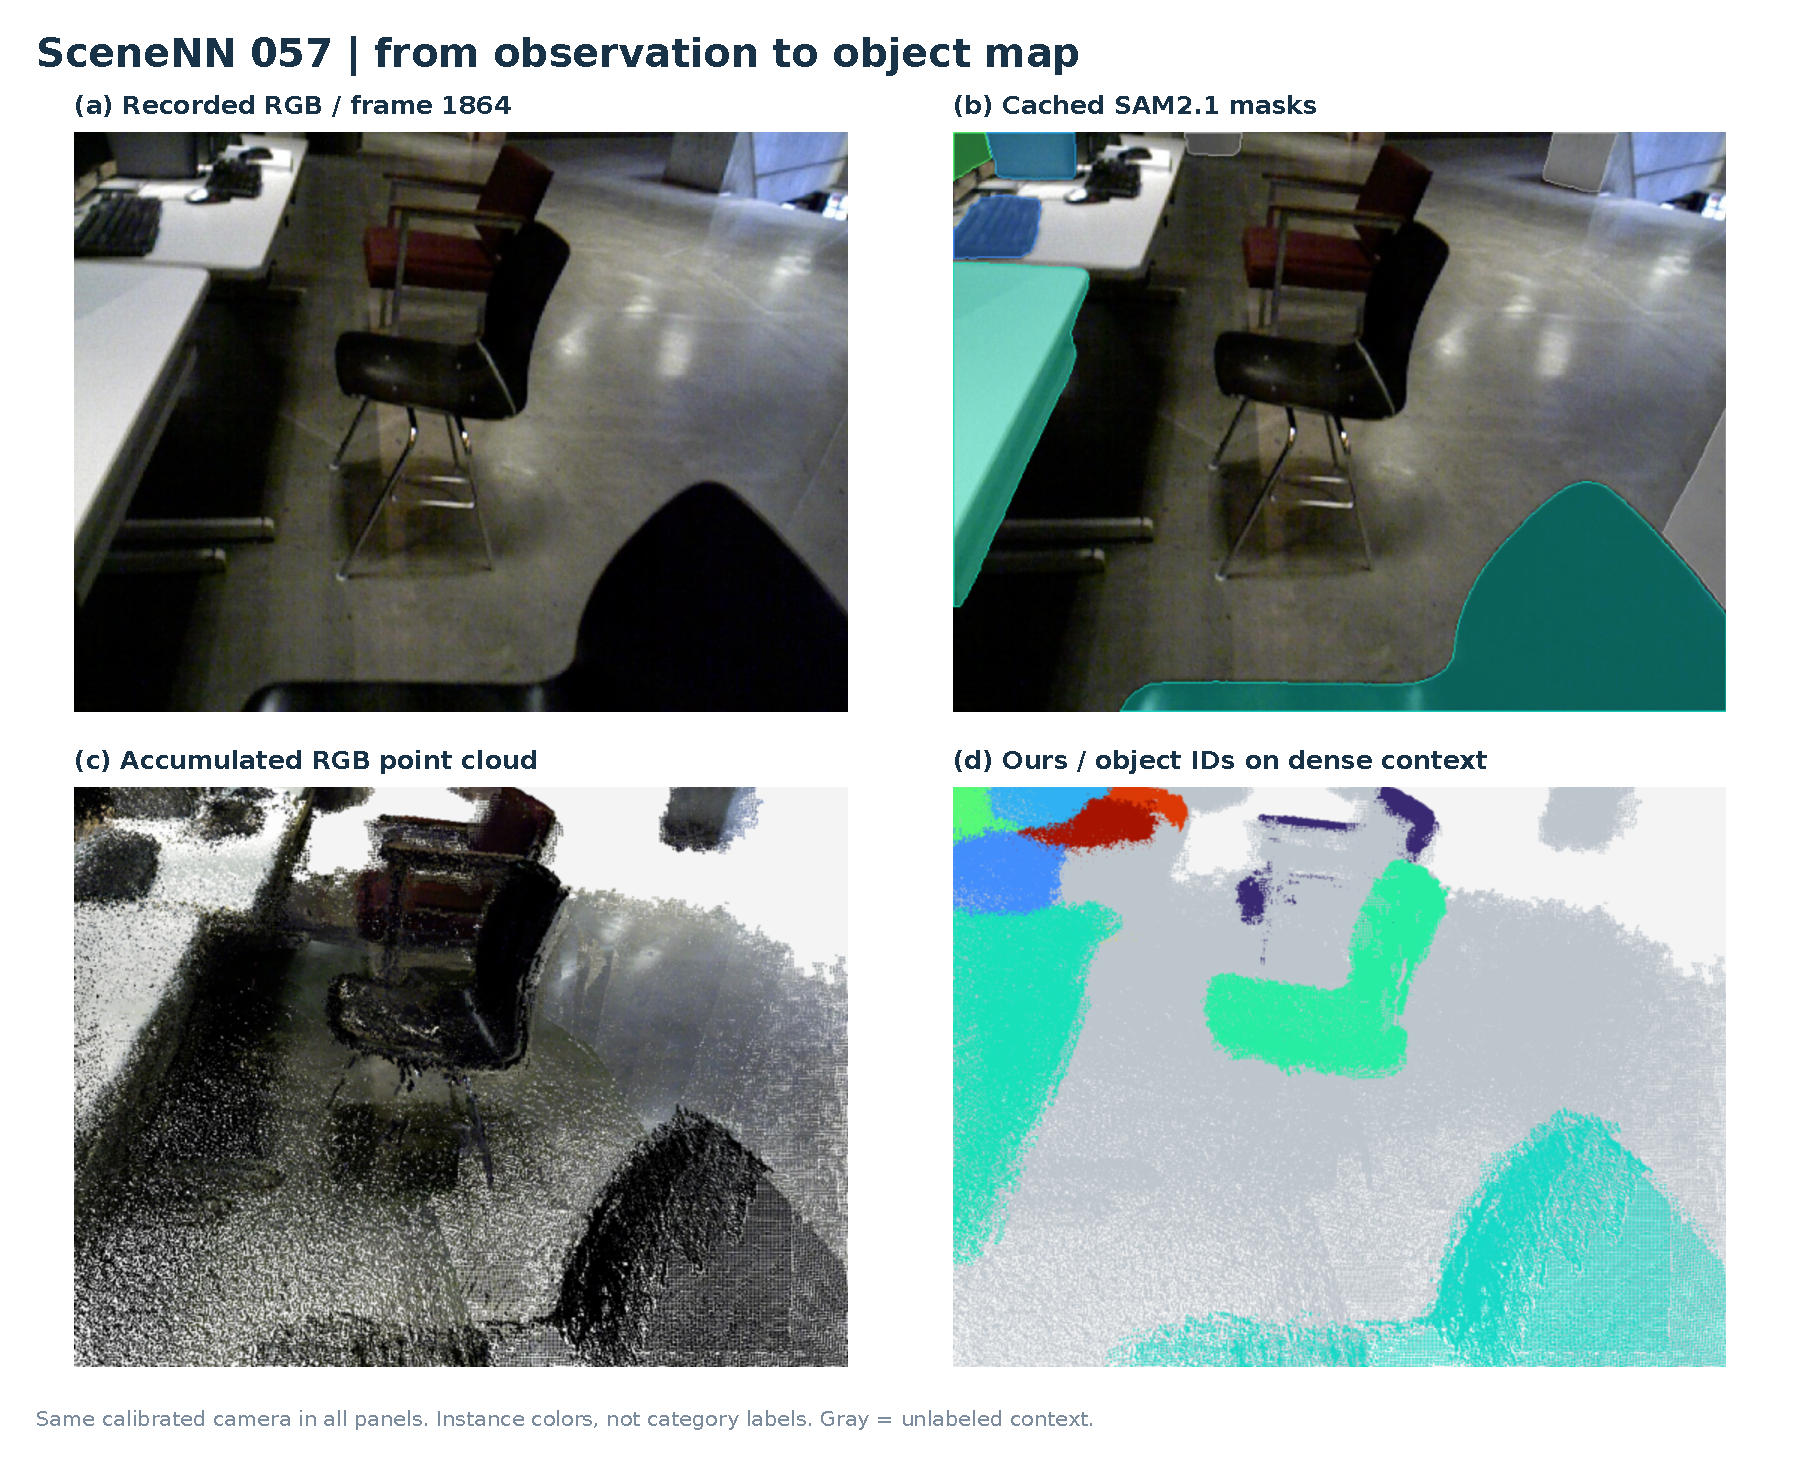
\includegraphics[width=.98\textwidth,height=.77\textheight,keepaspectratio]{dataset_scene_057.pdf}
\captionof{figure}{Actual RGB, cached SAM2.1 masks, accumulated colored geometry, and the V1 object map in one calibrated camera view. Embedded ``Ours'' means V1. The view was selected after evaluation to maximize support for predicted object 7. Point clouds use nearest-depth splats without hole completion. For dense display only, IDs transfer within 3\,cm; scoring uses 5\,cm on the observed-valid domain. Gray indicates unlabeled context. Colors encode predicted IDs, not GT classes.}
\end{center}

\clearpage
\section{SceneNN 061: A Second Evaluated V1 Scene}
\begin{center}
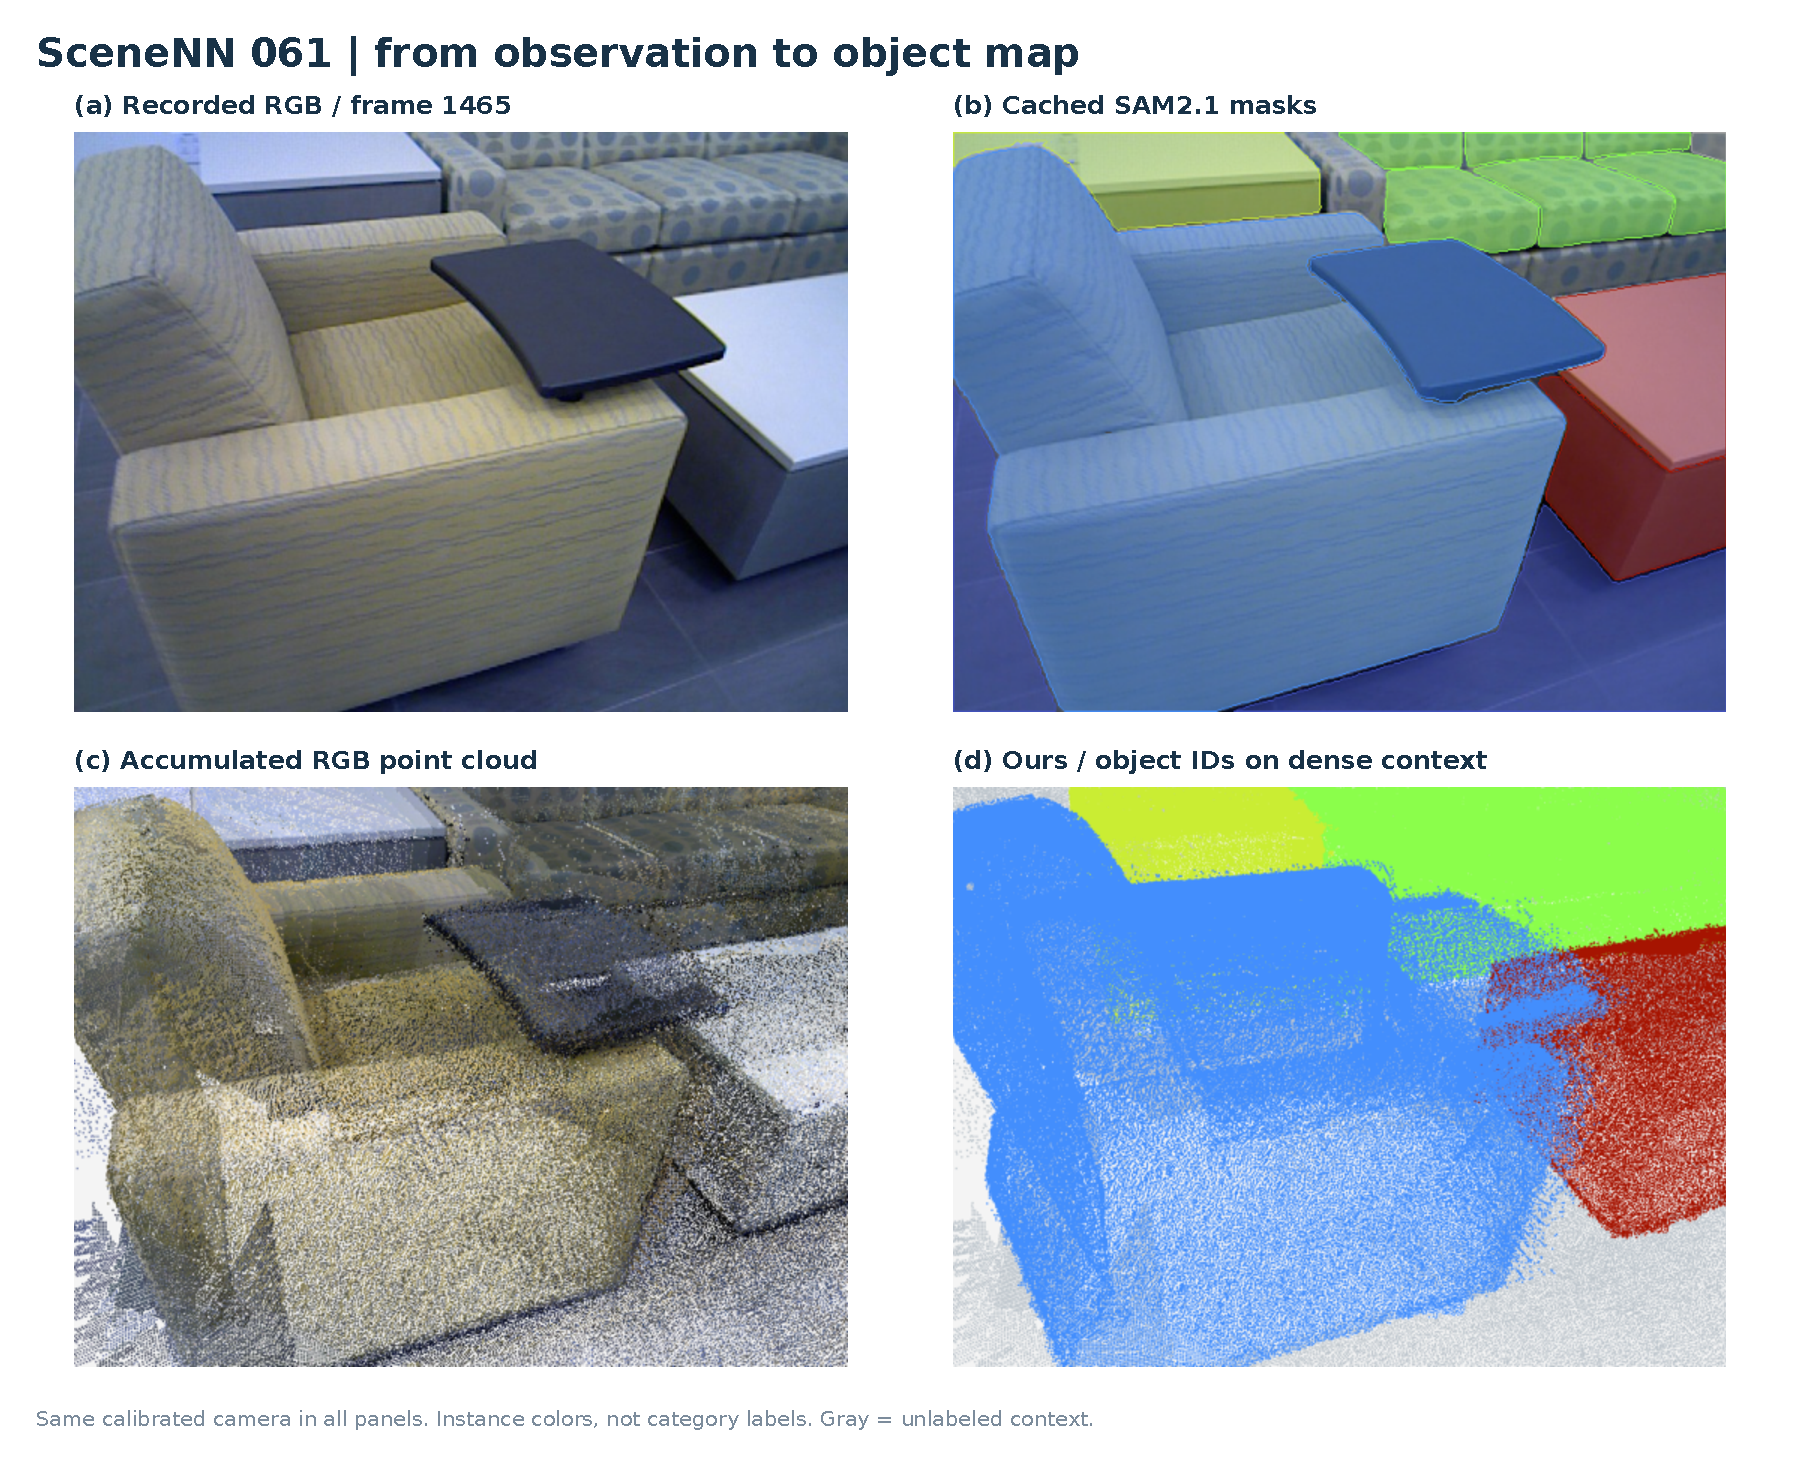
\includegraphics[width=.98\textwidth,height=.77\textheight,keepaspectratio]{dataset_scene_061.pdf}
\captionof{figure}{Real RGB and segmentation of the seating area, accumulated colored geometry, and V1 object IDs. Embedded ``Ours'' means V1. Display rules match the preceding page; the explanatory view maximizes cached support for predicted object 10. Accumulated geometry includes other viewpoints, so coverage need not match the single image. These are retained V1 results, not current-method cross-dataset runs.}
\end{center}
\clearpage
\section{V1 Development Gains and All-Object Changes}
The original development and new-scene plots are retained together with their exposure boundaries. ``Ours'' inside both plots denotes V1. The numerical tables and original predictions are unchanged.
\begin{center}
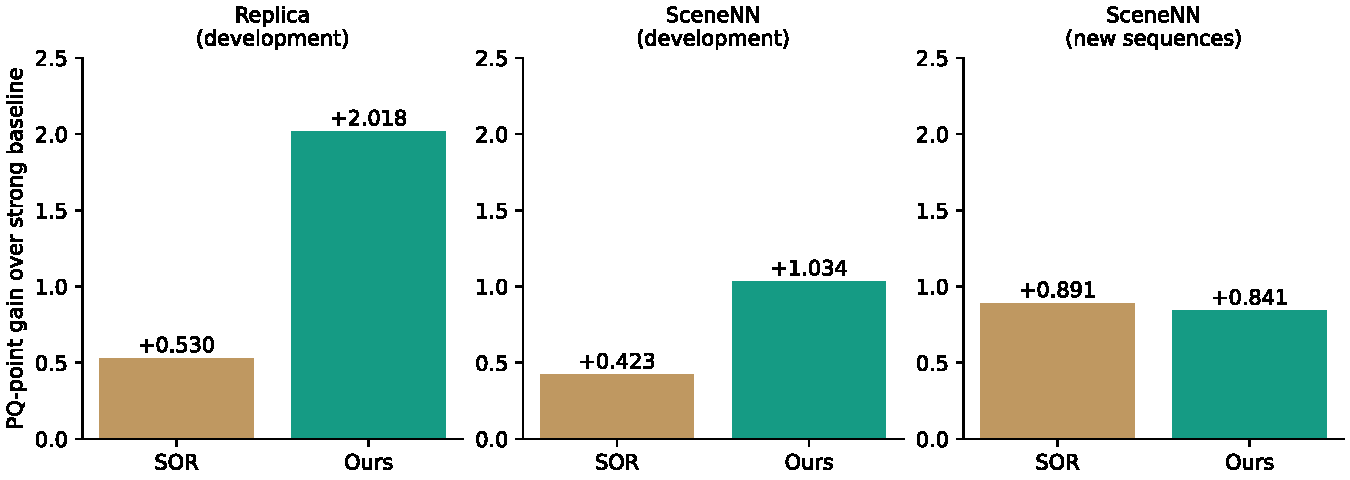
\includegraphics[width=\textwidth]{development_vs_unseen.pdf}
\captionof{figure}{PQ-point gains over the corresponding strong baseline, separated by dataset and development exposure. Replica office\_0/office\_1 and SceneNN 014/015 were exposed development scenes. Only the final group is the four new SceneNN sequences in the V1 main table. These gains do not describe current KITTI-360 authorization.}
\end{center}
\begin{center}
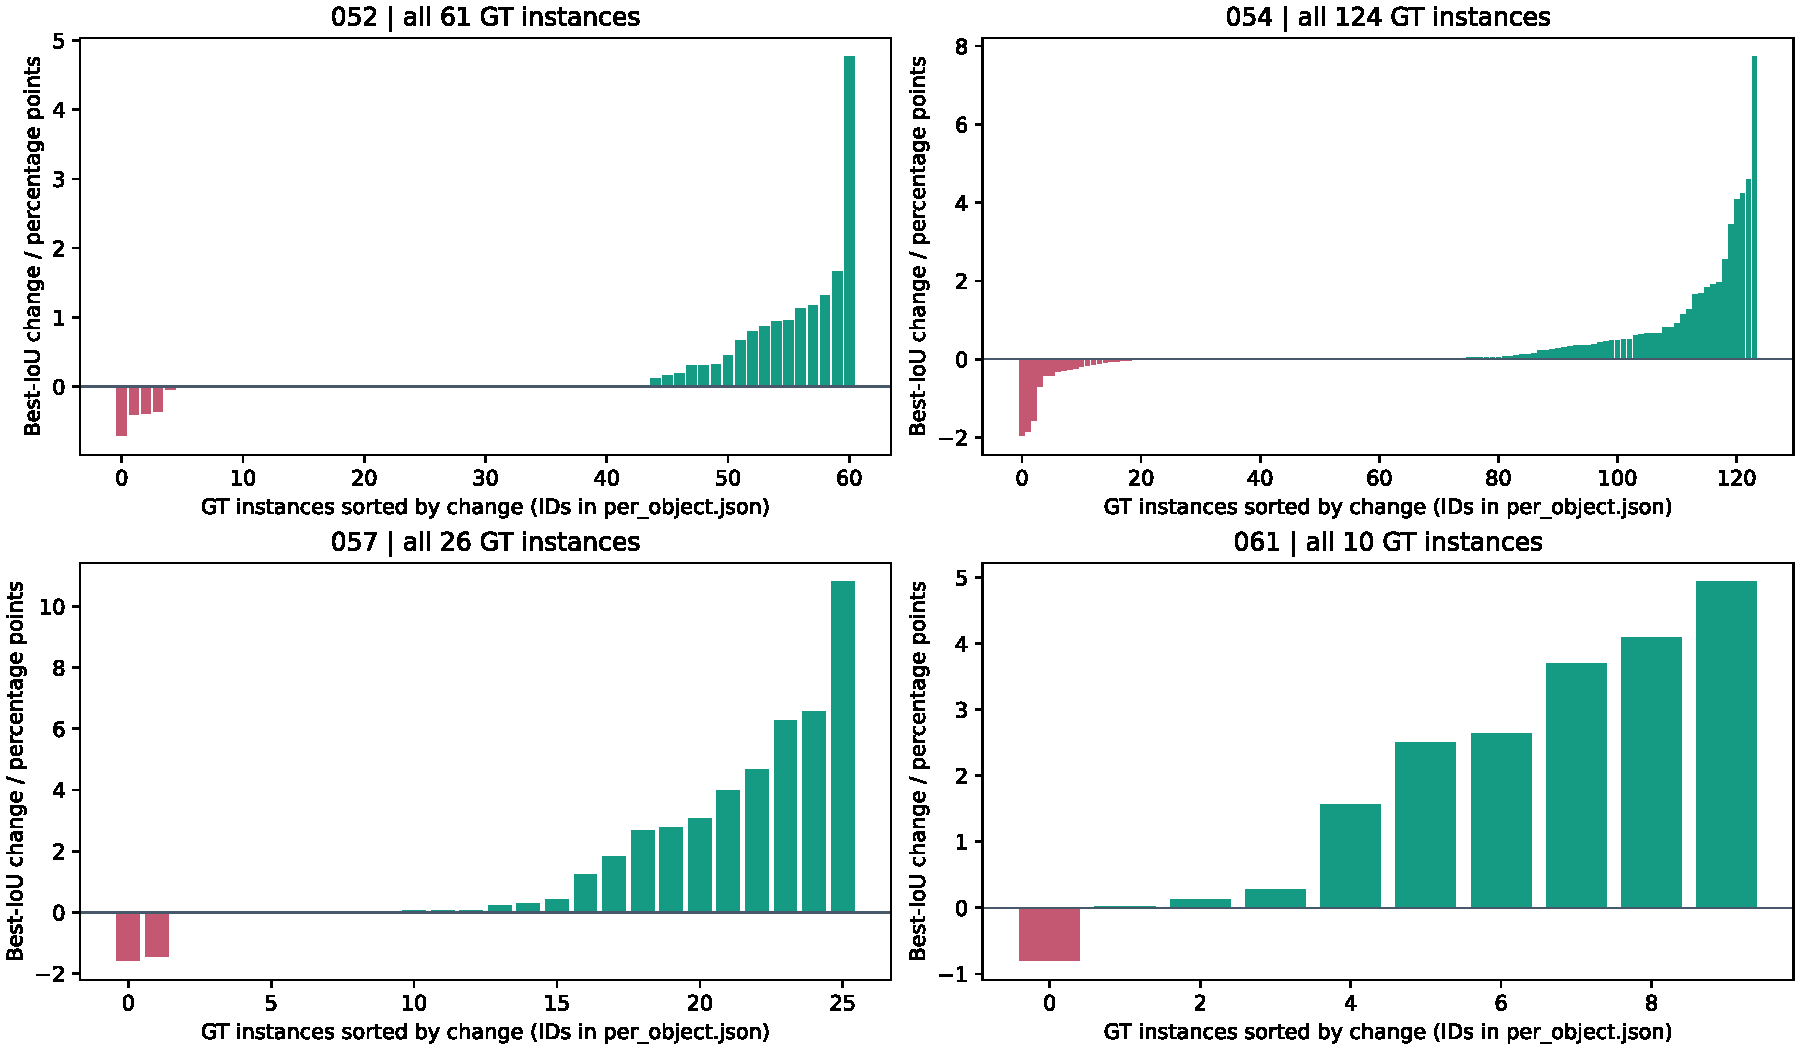
\includegraphics[width=\textwidth]{all_object_changes.pdf}
\captionof{figure}{Best-object IoU changes for all 221 GT instances in the four V1 SceneNN sequences. Objects are sorted by change within each scene; unchanged and regressed instances remain visible. There are 100 improvements, 27 declines, and 94 unchanged objects. Objects within a scene are not independent statistical trials.}
\end{center}

\clearpage
\section{V1 Evidence and Assignment Diagnostics}
These diagnostics explain why the V1 sequence-057 result trails SOR even though many individual geometries improve. They retain the original metric and the separately labeled locked-assignment diagnostic.
\begin{center}
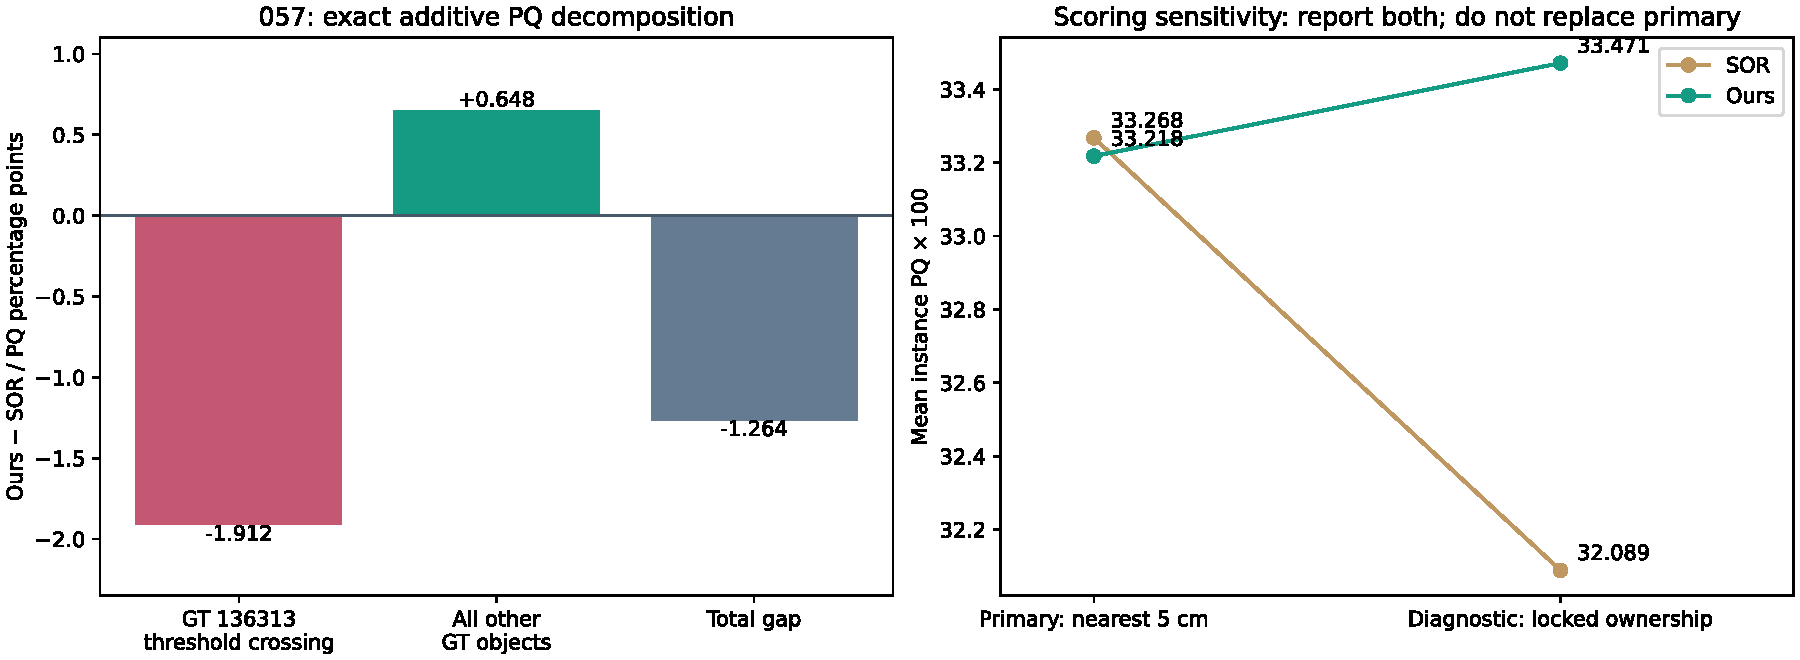
\includegraphics[width=\textwidth]{mechanism_decomposition.pdf}
\captionof{figure}{V1 sequence-057 primary-score deficit relative to SOR: one SOR-only match outweighs gains on the remaining objects. Locking baseline source ownership changes the mean ranking across four scenes. Locked assignment probes reference-label reassignment; it does not replace primary nearest-source evaluation. Embedded ``Ours'' means V1.}
\end{center}
\begin{center}
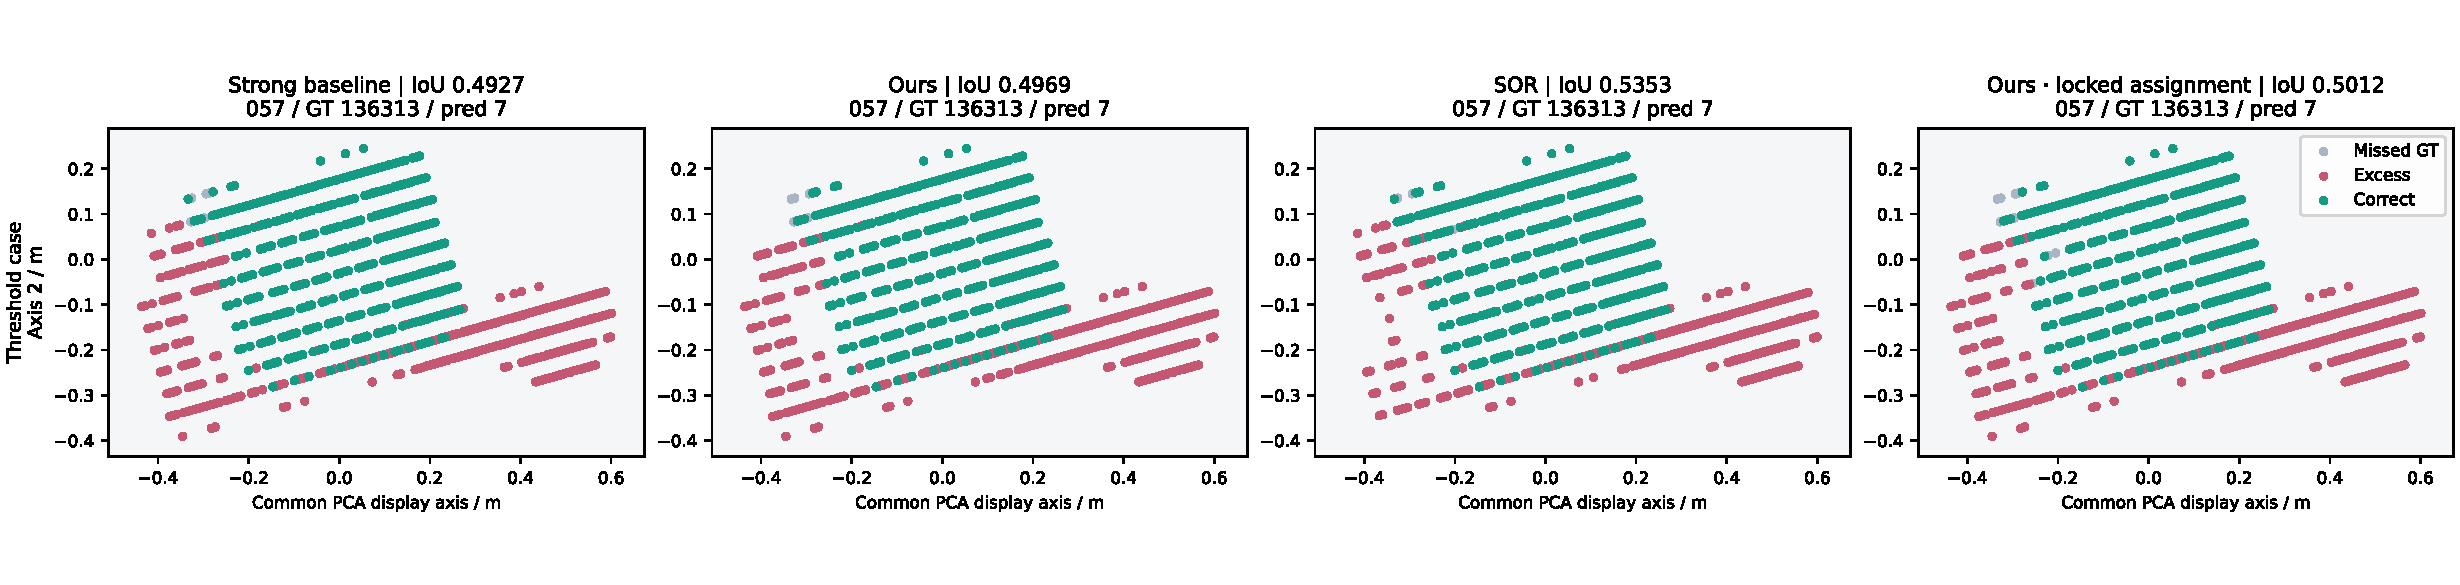
\includegraphics[width=\textwidth]{057_threshold_case.pdf}
\captionof{figure}{Threshold-sensitive GT object 136313 in a shared projection. Correct, excess, and missed reference support are green, red, and gray. The fourth panel locks baseline nearest-source ownership before deletion. All panels show the archived V1 study; ``Ours'' and ``Ours + locked assignment'' are not current-method results.}
\end{center}
The primary IoUs are 0.492718 (strong baseline), 0.496947 (V1), and 0.535340 (SOR). The locked V1 diagnostic is 0.501247. This case illustrates a threshold and ownership interaction, rather than evidence that deleting more points is necessarily better.

\clearpage
\section{Archived Garage Objects and Visual Evidence}\label{app:archived-garage}
\begin{center}
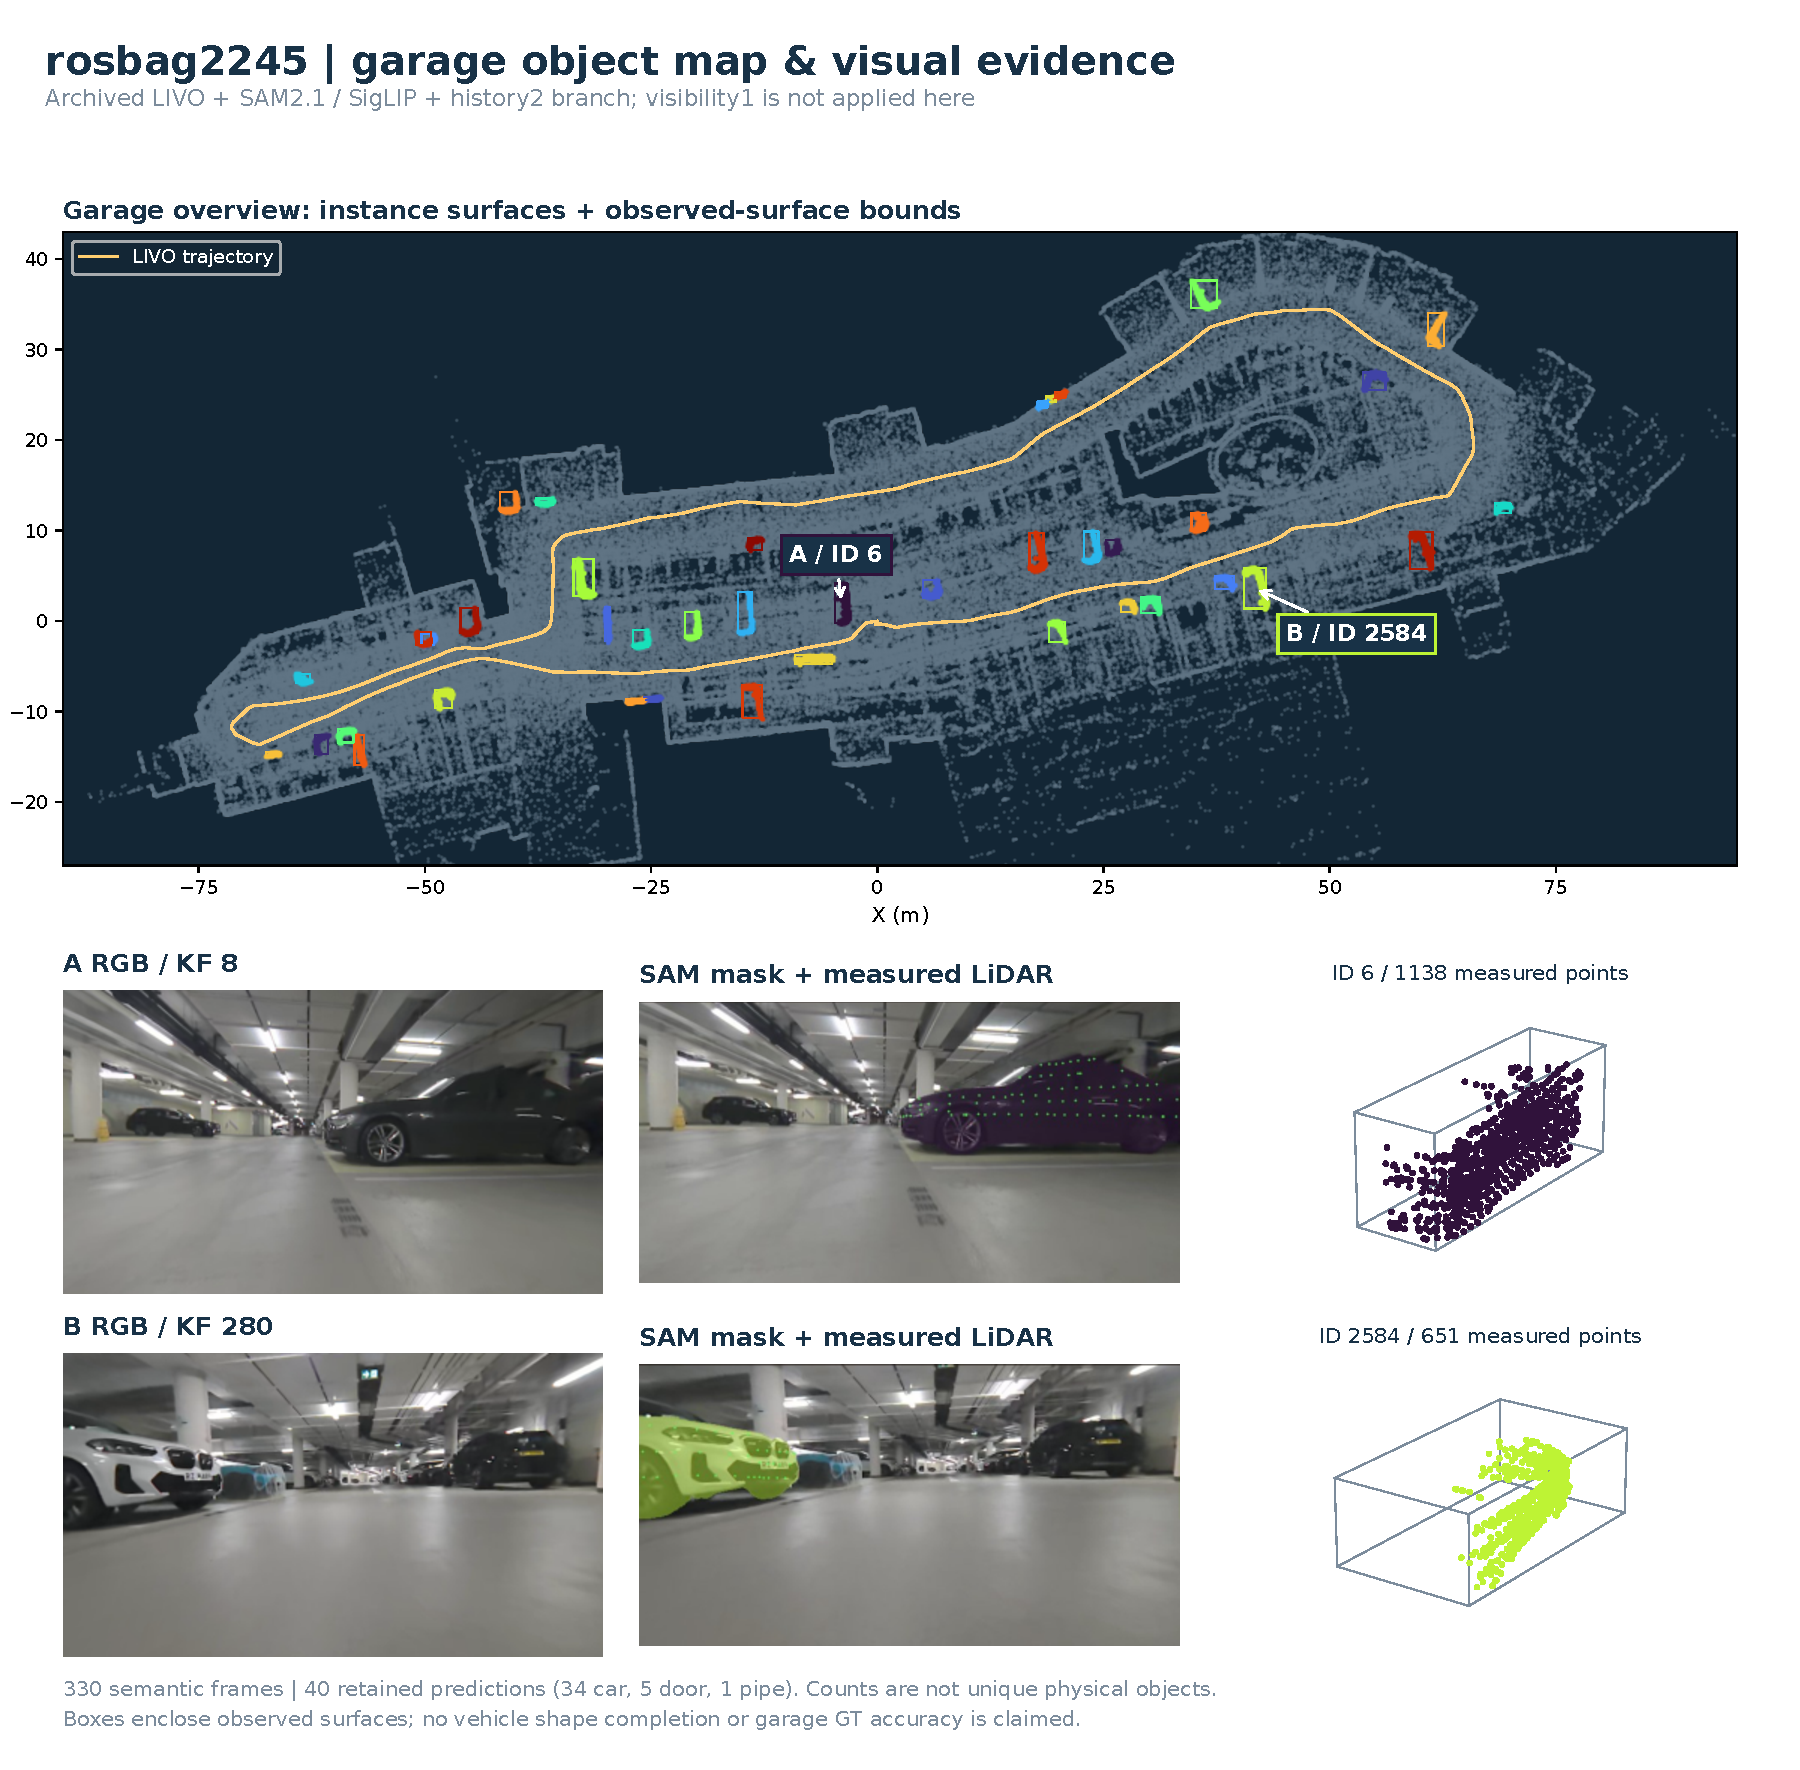
\includegraphics[width=.98\textwidth,height=.76\textheight,keepaspectratio]{garage_real_evidence.pdf}
\captionof{figure}{Archived \texttt{rosbag2245} LIVO + SAM2.1/SigLIP + history2 replay. The map links vehicle records to actual RGB, masks, measured LiDAR support, and accumulated surfaces with boxes. The overview shows all 40 retained predictions with the original crop and context subsampling. Its 330 cached frames produce 34 car, five door, and one pipe records; these are prediction records, not verified unique physical objects. Boxes bound observed surfaces. Neither V1 nor current authorization was applied to this archived map.}
\end{center}
This is the original garage object-evidence view in its own \texttt{omni\_odom} coordinates. It complements the current four-method garage comparison in Appendix~\ref{app:robot}; overlays and IDs are not transferred between these map revisions.


\clearpage
\section{Archived Robot Recordings and Garage Routes}\label{app:routes}
\begin{center}\small
\begin{tabular}{lrrr}
\toprule
Recording & Minutes & Path (m) & Map points \\
\midrule
roabag2336 & 3.1 & 84.5 & 178,179 \\
rosbag0521\_2 & 4.0 & 108.8 & 199,568 \\
rosbag2245 & 9.8 & 316.2 & 565,791 \\
rosbag2\_20260415\_174148 & 18.9 & 556.9 & 2,148,498 \\
20260414\_4 & 24.3 & 838.4 & 2,778,455 \\
rosbag2\_20260415\_162852 & 27.4 & 834.9 & 3,063,285 \\
\bottomrule
\end{tabular}

\captionof{table}{Original six-recording inventory. Path lengths are trajectory estimates, not ground truth; map point counts belong to the reviewed geometric-map revision, not the current semantic output.}
\end{center}
Recordings may revisit the same sites. They are not six independent semantic tests. Atlas point colors encode height, with deterministic subsampling and central 99\% XY display extent; each route has its own scale. These reviewed offline-backend coordinates are not mixed with later garage or outdoor semantic-map revisions.
\begin{center}
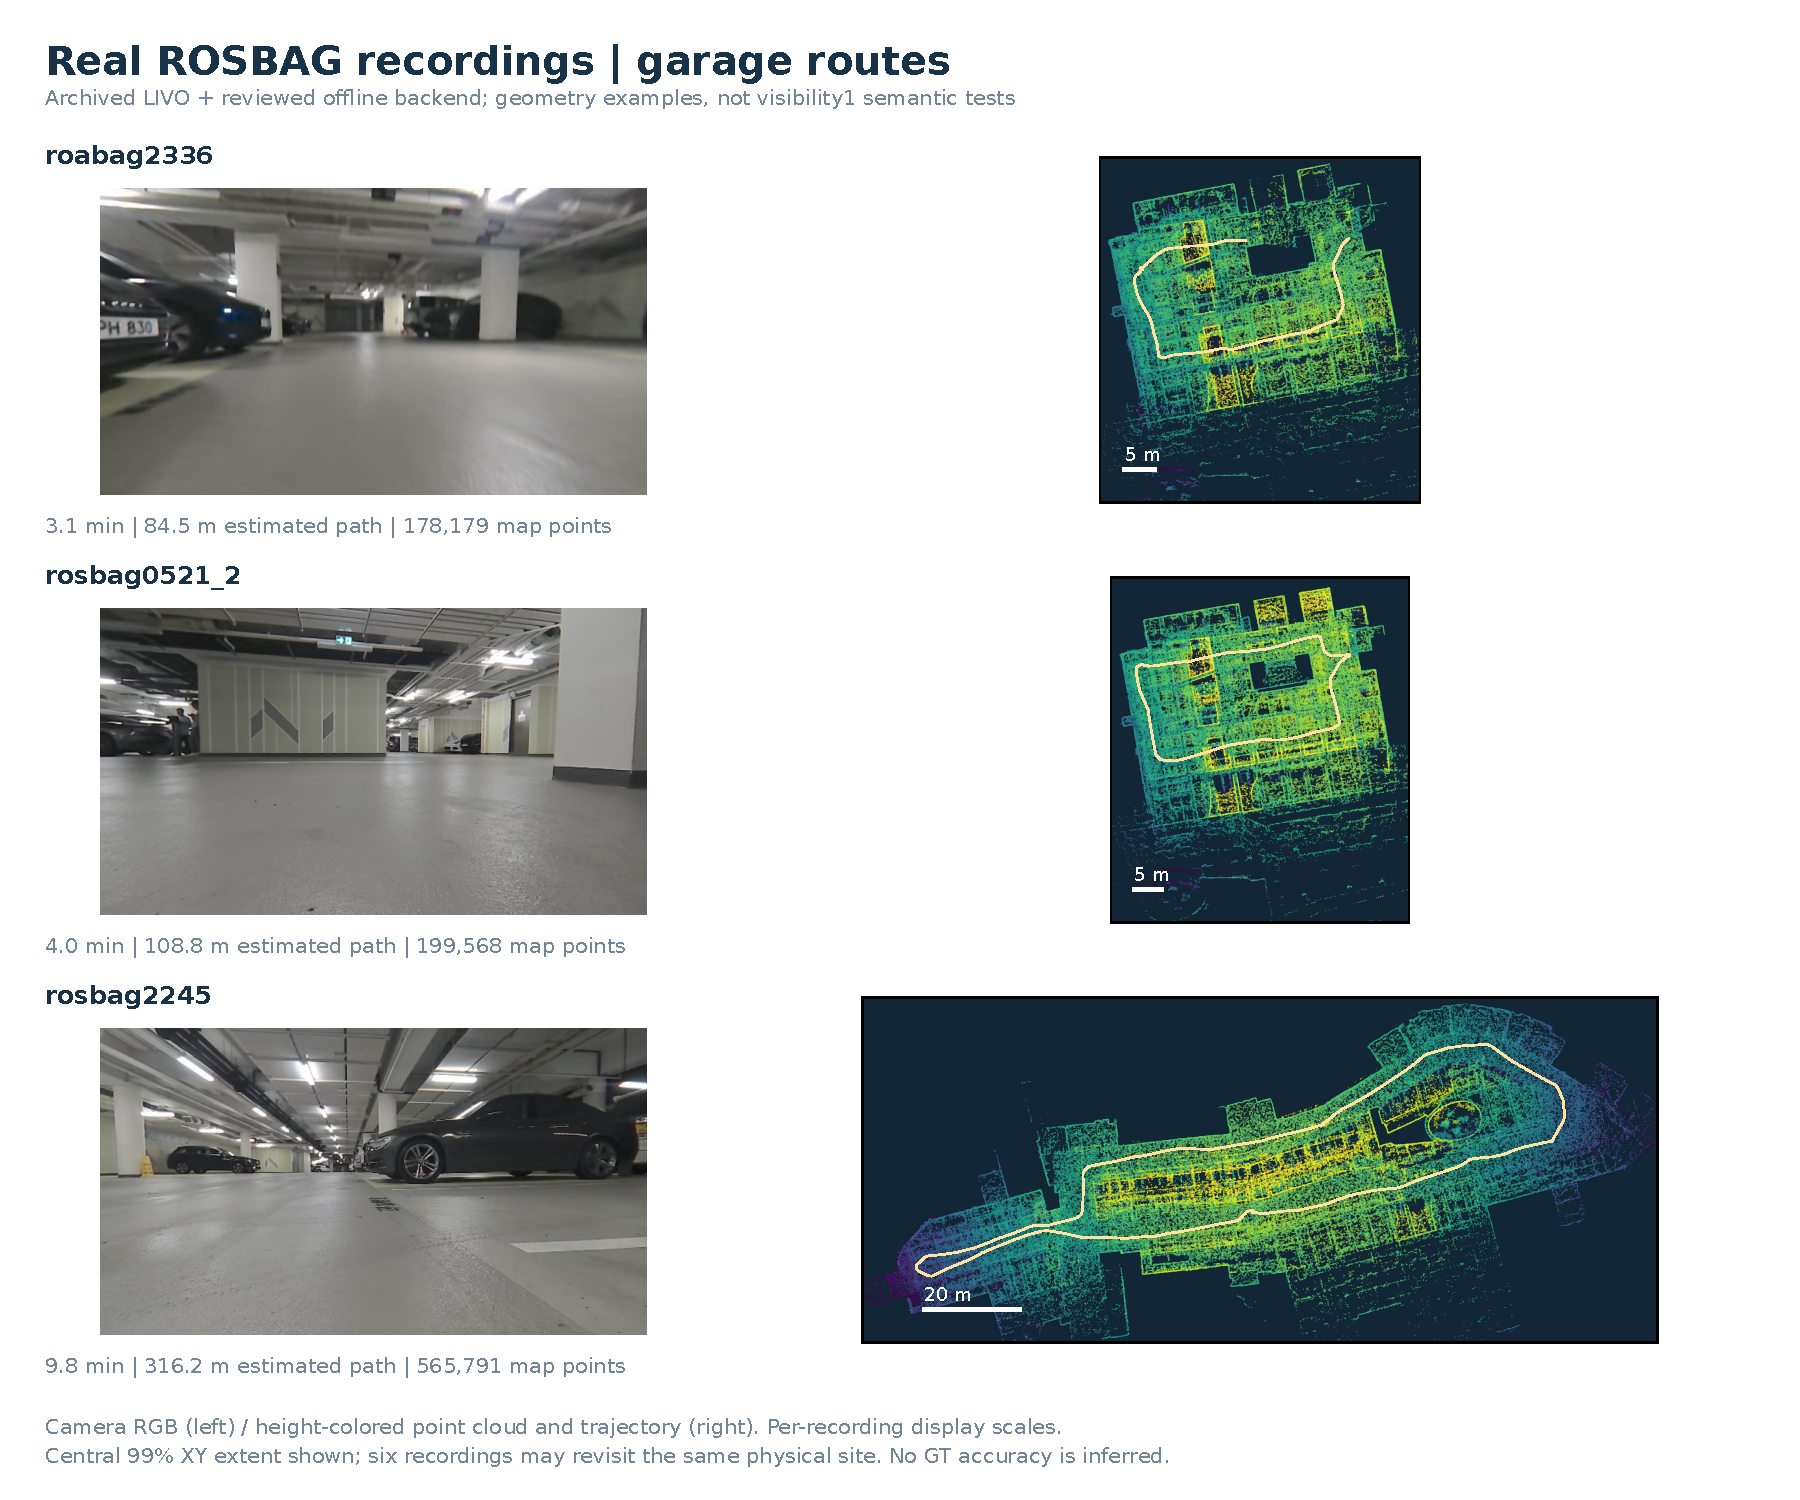
\includegraphics[width=.96\textwidth]{rosbag_routes_1.pdf}
\captionof{figure}{Three actual garage recordings: undistorted camera views, height-colored LiDAR maps and estimated trajectories. These archived sensing results predate the current revision comparison.}
\end{center}
The separate current garage comparison uses the sealed 330-frame semantic branch and the same authorization kernels as the new public assessment. Its results are reported in Appendix~\ref{app:robot}, not inferred from this atlas or its point counts.

\clearpage
\section{Archived Outdoor Routes}
\begin{center}
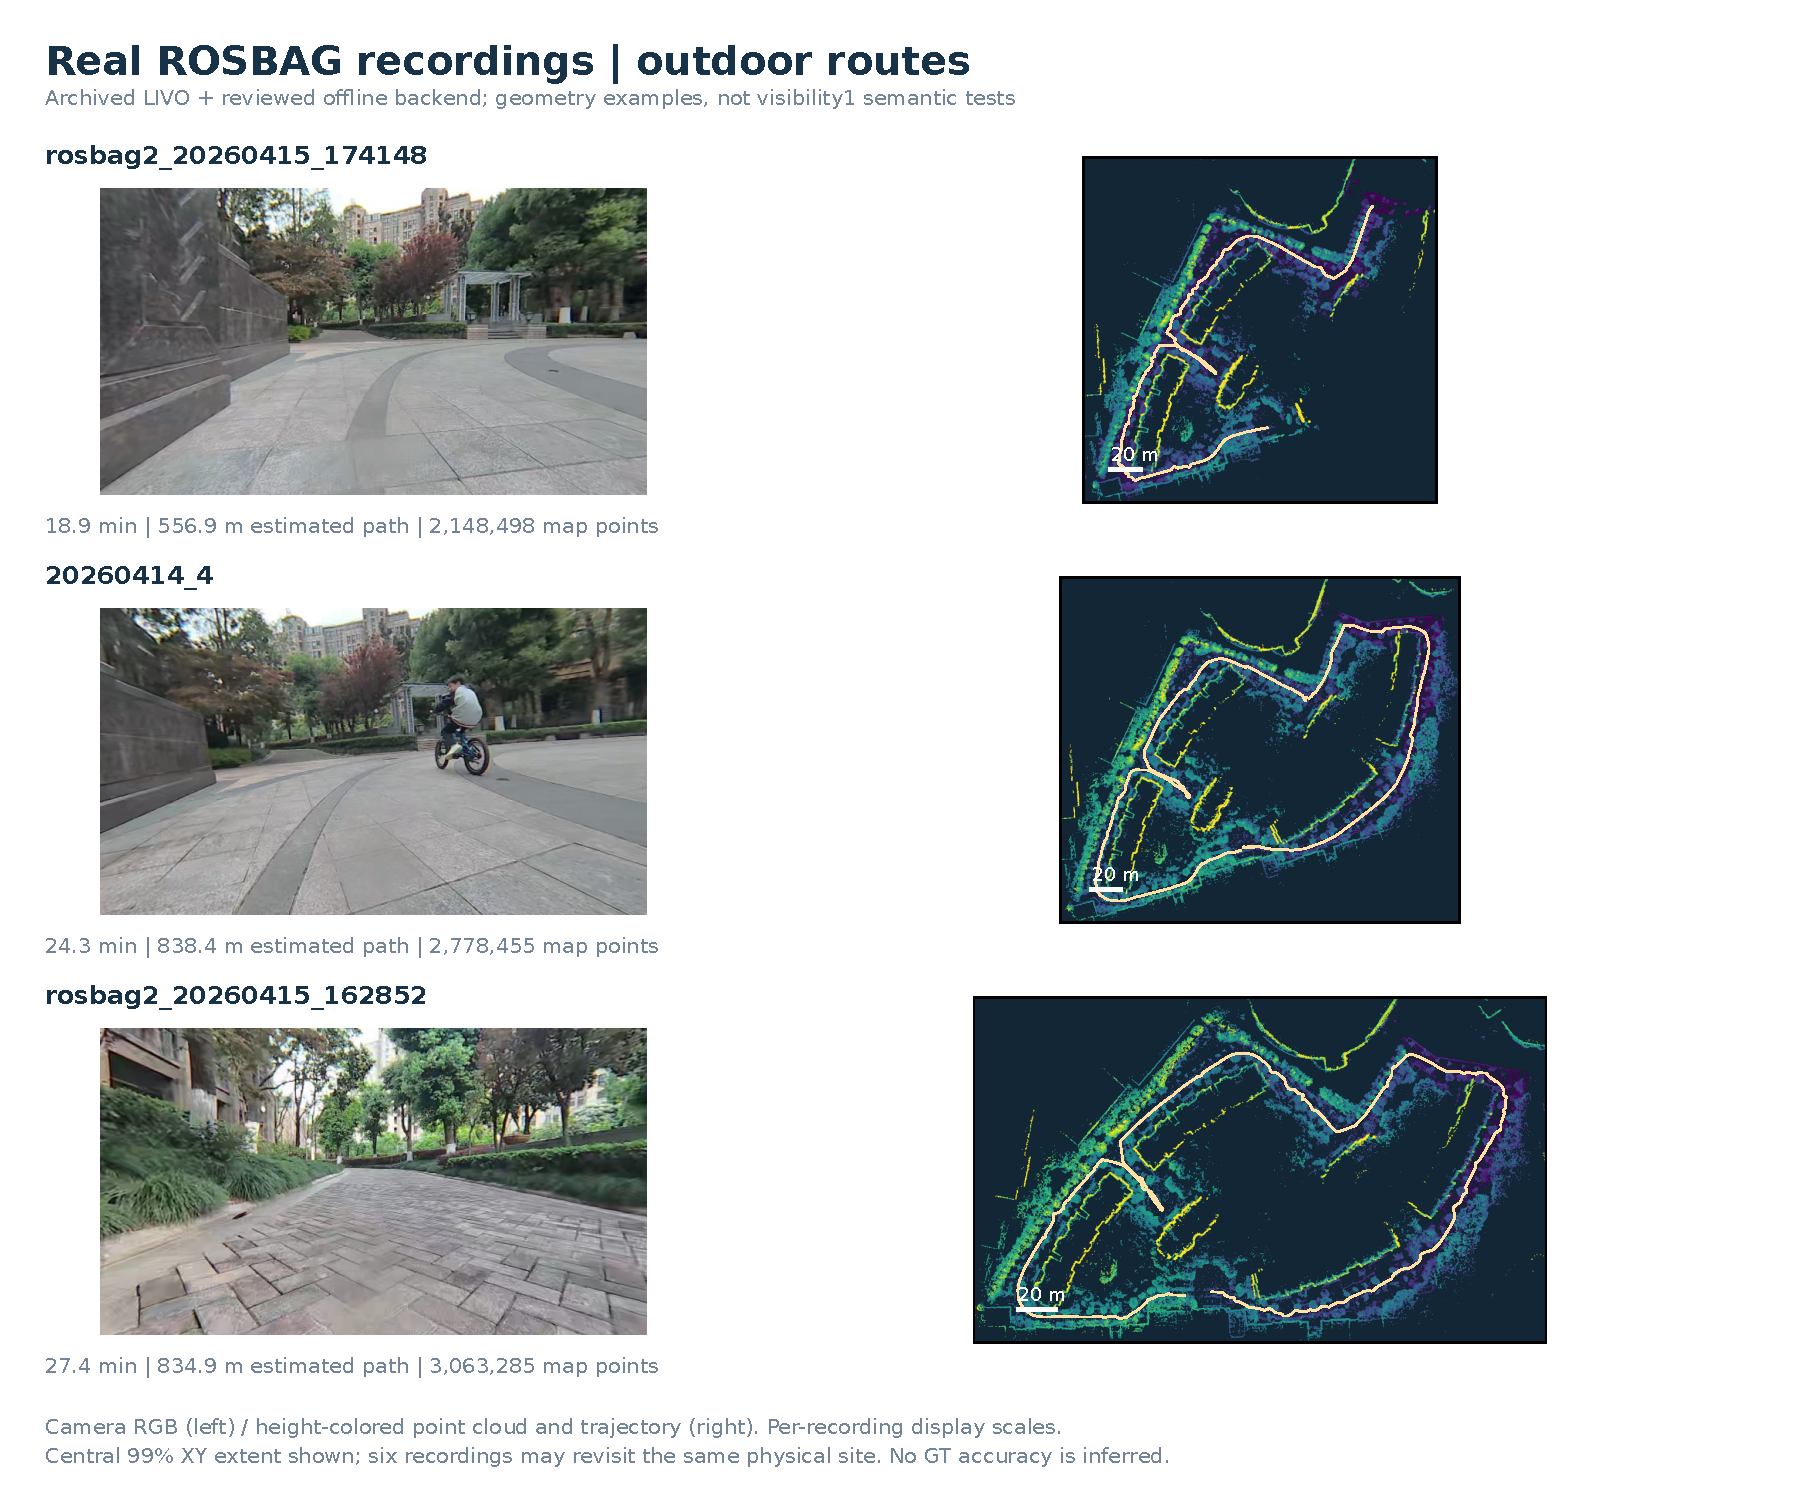
\includegraphics[width=.98\textwidth]{rosbag_routes_2.pdf}
\captionof{figure}{Three actual outdoor recordings, including estimated paths around 835 and 838\,m. Height colors and per-recording scales match the garage atlas conventions. Spatial overlap is possible; neither independent-site generalization nor current-method semantic accuracy follows.}
\end{center}
\subsection{System and map-version provenance}
The outdoor semantic record \texttt{rosbag2\_20260415\_162852} contains 440 keyframes. Grounding DINO tiny produces image detections, followed by measured-depth association. The archived static map retains 19 repeated-observation records (15 plant and four door/entrance candidates). These counts are prediction records, not verified unique physical objects. SegFormer B0 with Cityscapes weights proposes image-level ground support; local geometric checks select measured LiDAR points.

The original garage object-evidence branch uses its own \texttt{omni\_odom} coordinates and retained 40 records (34 cars, five doors, one pipe) under SAM2.1/SigLIP/history2. It differs from both the geometric-route atlas and the current 68-ID authorization output. No detections, boxes, masks, or trajectories are transferred between these revisions in this document.

The following pages retain the outdoor landmark and ground examples from their internally consistent original revision. They show useful sensing and evidence interfaces. They are not additional evaluations of either V1 or current \ours{}, and no unannotated semantic-accuracy or real-time claim is attached to them.

\clearpage
\section{Archived Outdoor Landmarks and Measured Bounds}
\begin{center}
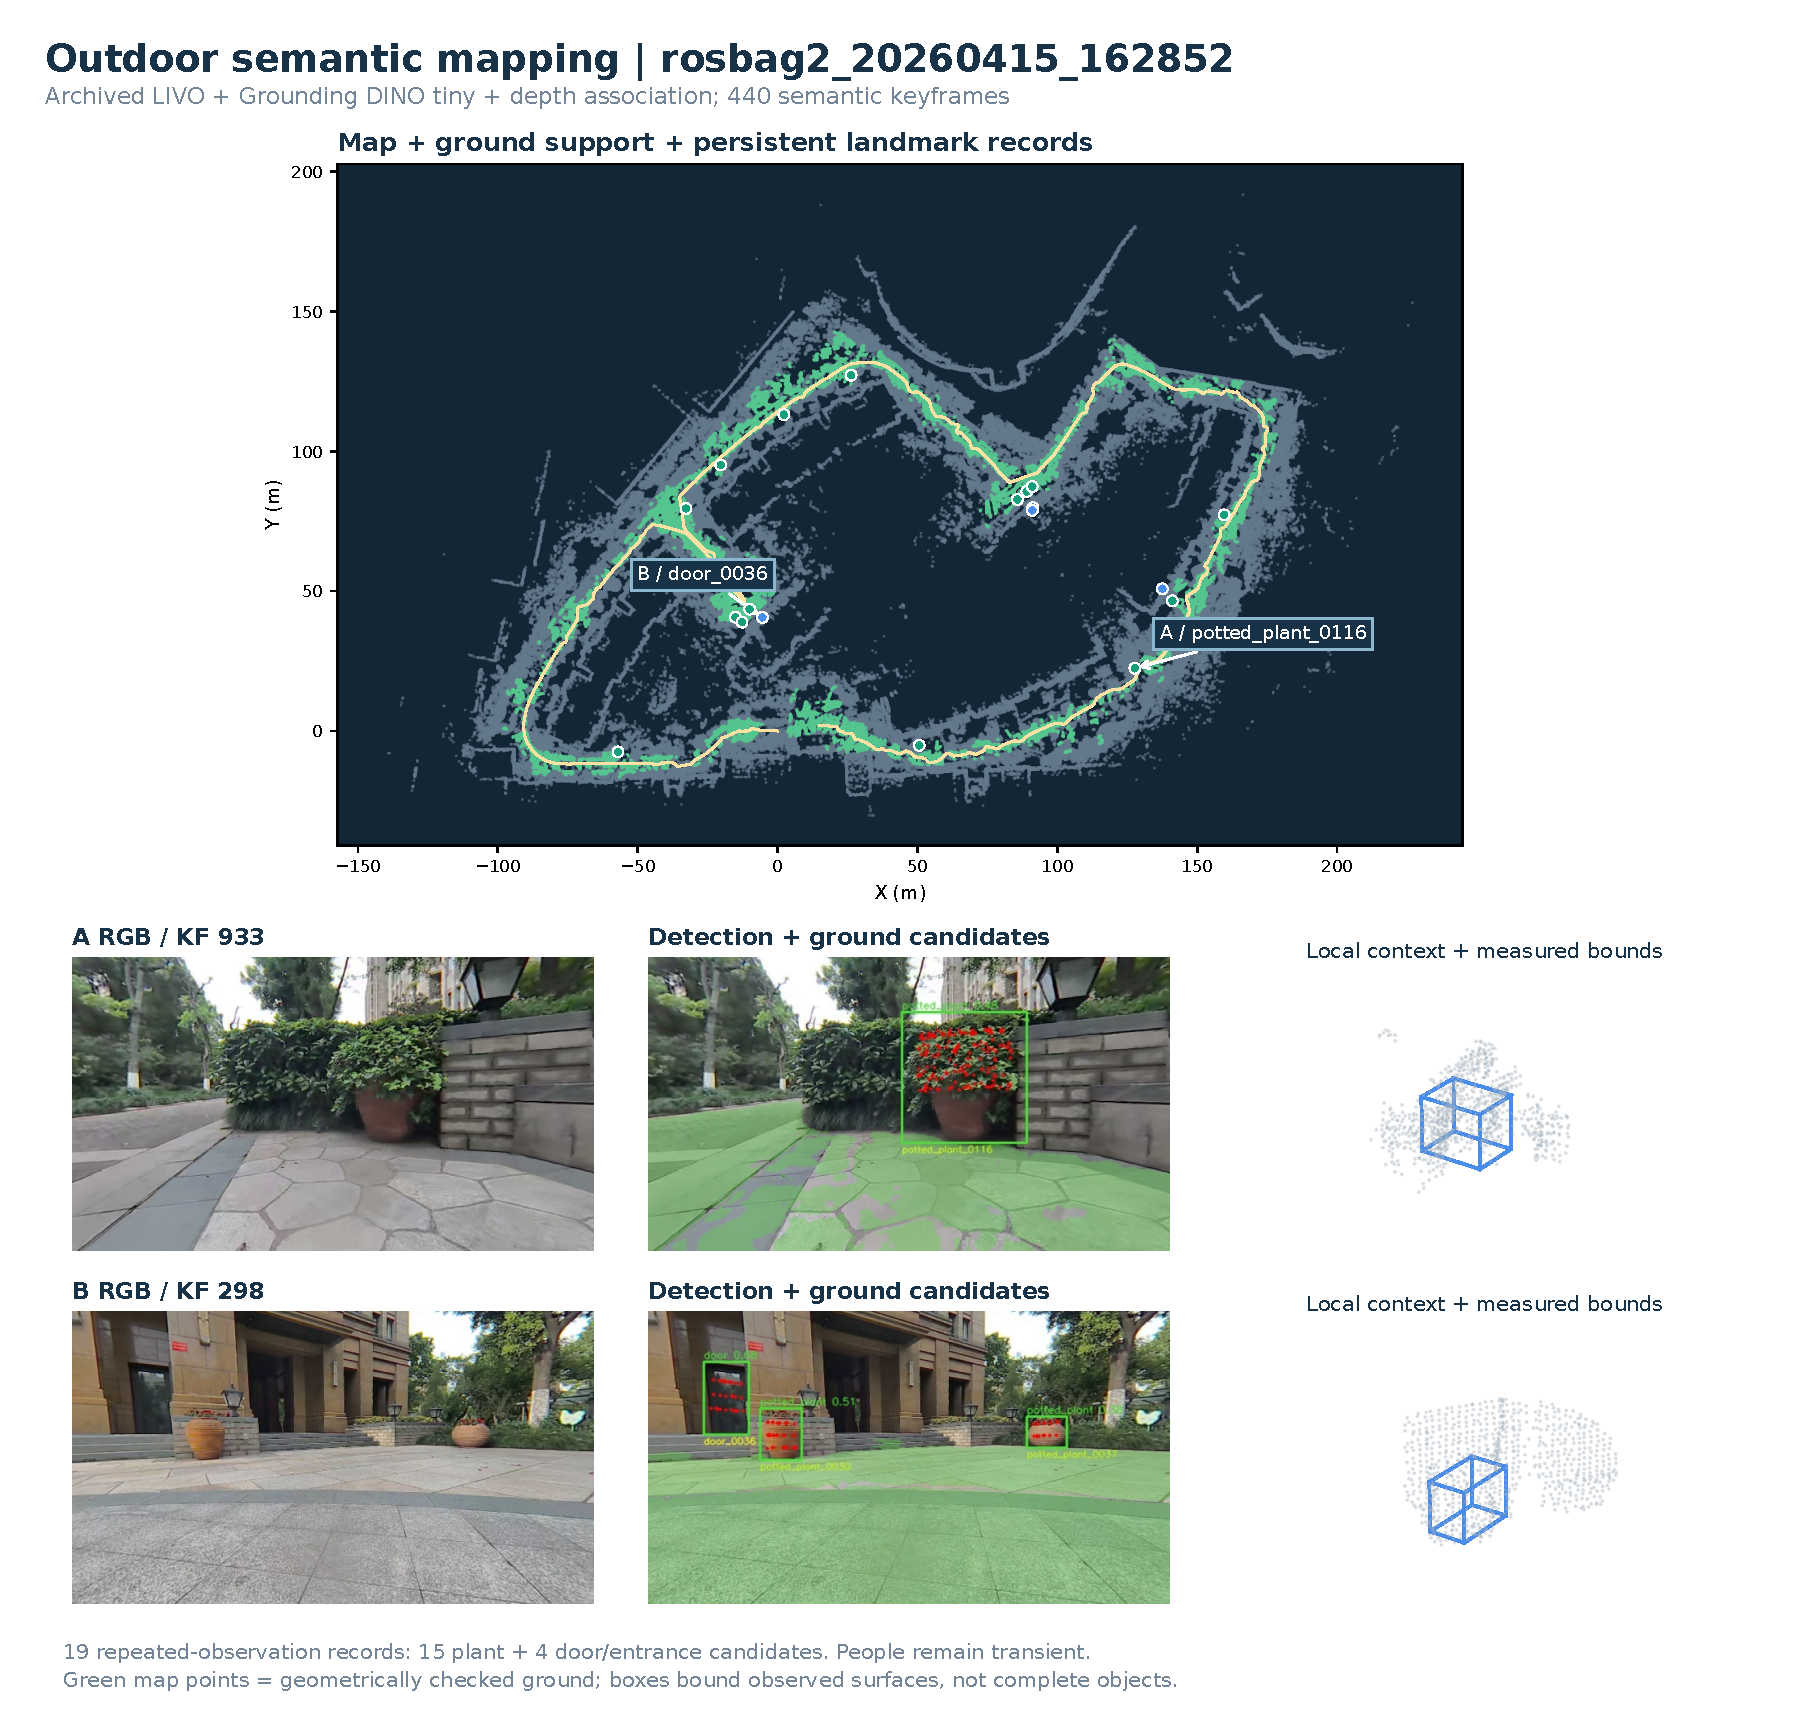
\includegraphics[width=.98\textwidth,height=.78\textheight,keepaspectratio]{rosbag_outdoor_semantics.pdf}
\captionof{figure}{Archived outdoor semantic map, route, checked ground support, and two selected records linked to real images and measured bounds. Gray local points are context, not isolated object geometry. Each record shows its largest observed image box. Categories and boxes are predictions; measured bounds are not independently evaluated 3D detections or full object shapes.}
\end{center}
These images and point clouds were retained without new inference. Coordinates are those of this archived outdoor semantic branch. The figure documents the observation-to-object interface; it does not establish a gain from the current revision module.

\clearpage
\section{Archived Ground and Transient Observations}
\begin{center}
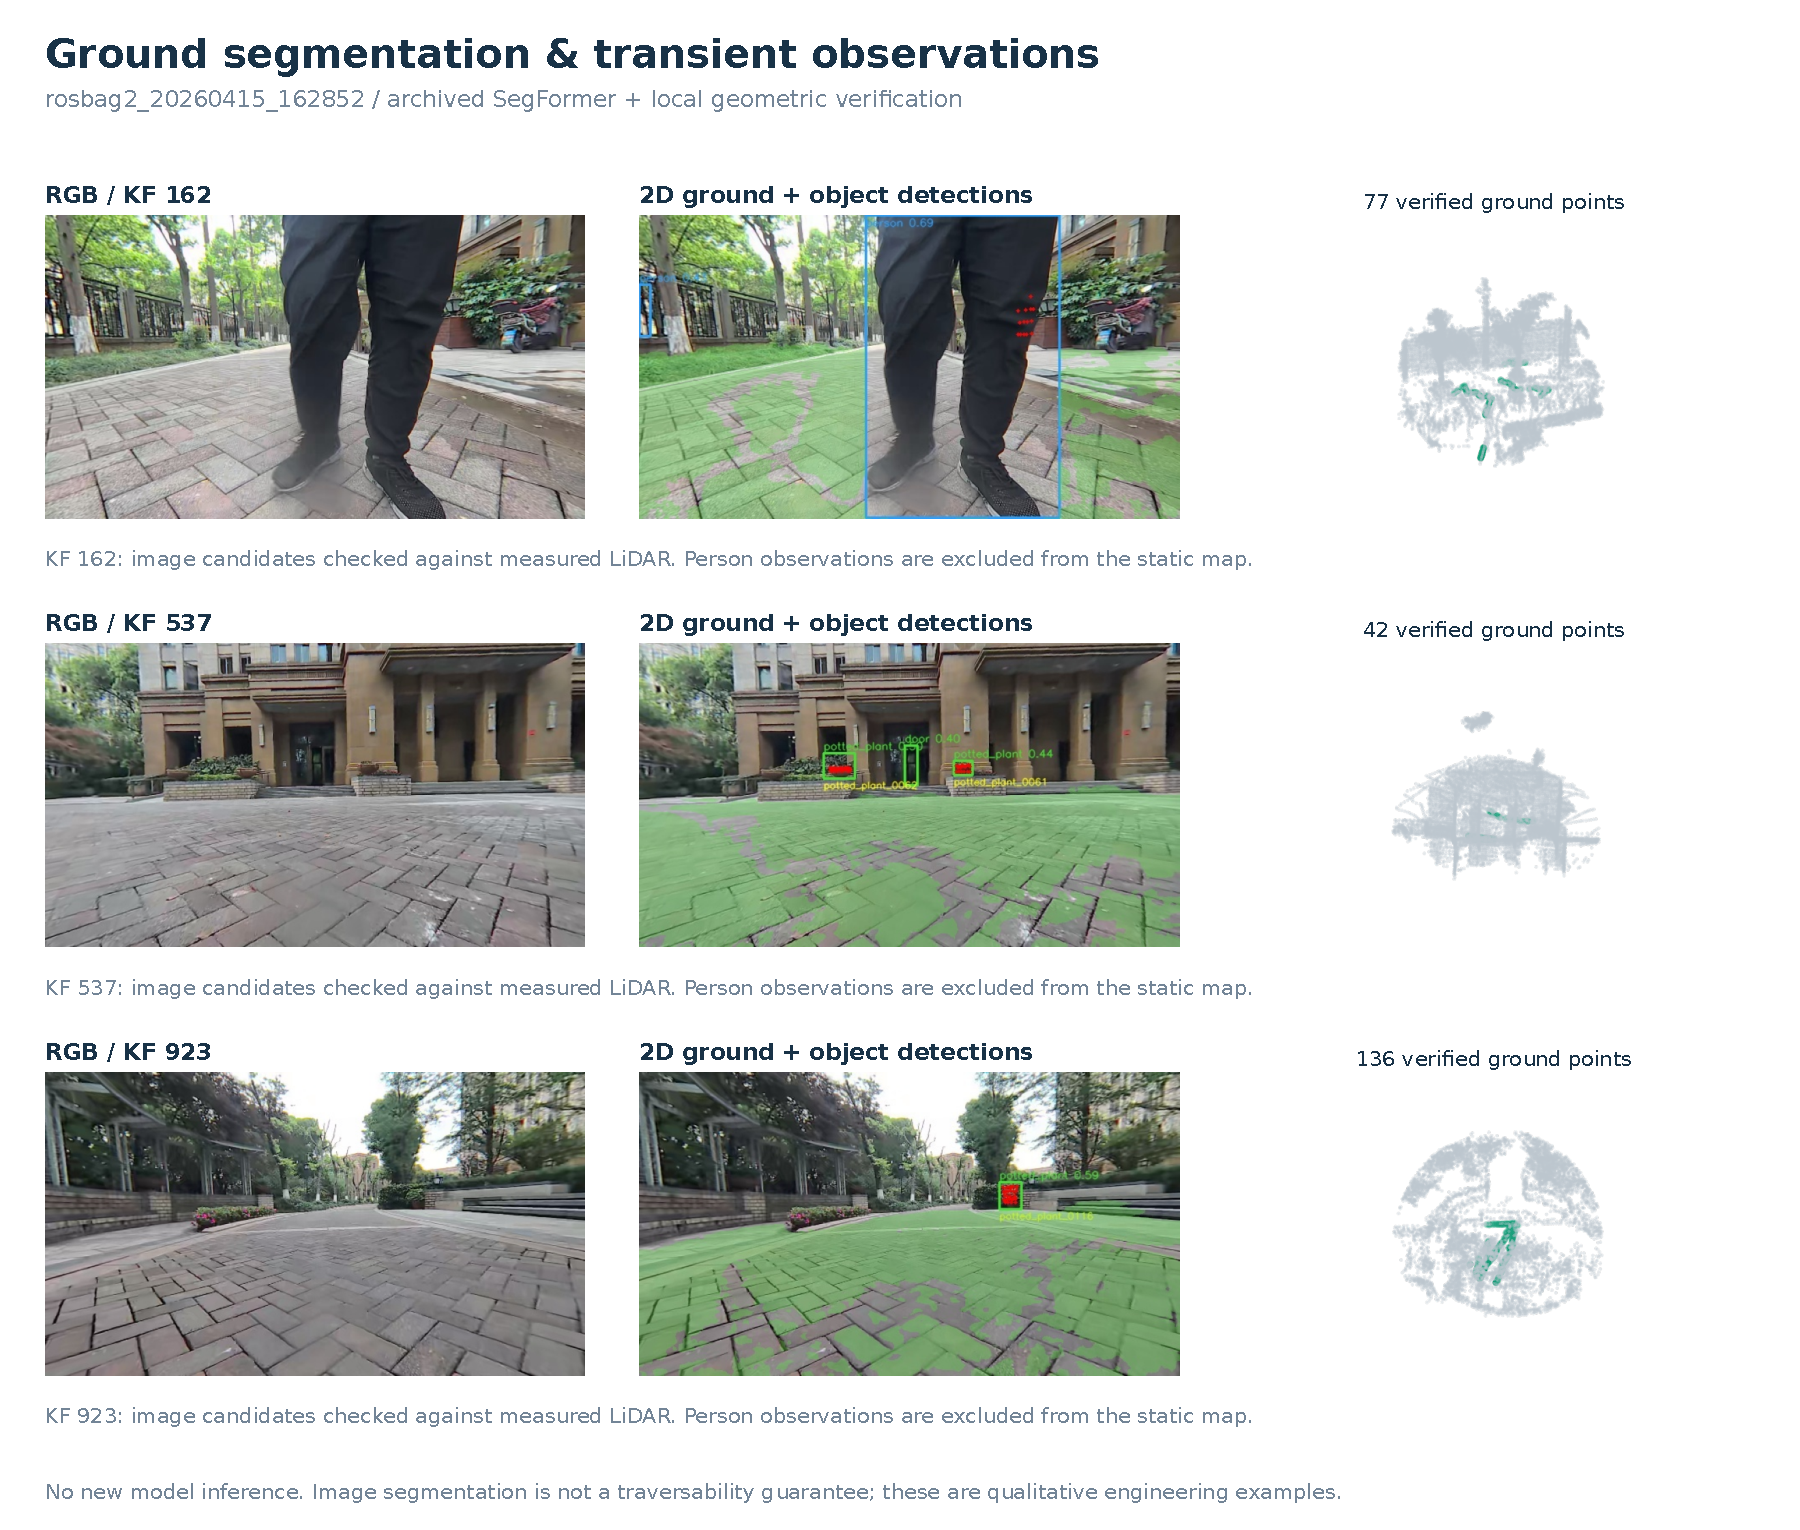
\includegraphics[width=.98\textwidth,height=.78\textheight,keepaspectratio]{rosbag_ground_details.pdf}
\captionof{figure}{Three actual outdoor keyframes: RGB, image-level ground candidates and detections, and geometrically checked LiDAR ground support. Image candidates and accepted 3D points are different outputs. Selected frames have nonempty accepted support; other frames may not. People remain transient observations and are excluded from static landmarks.}
\end{center}
These examples preserve the original scope: qualitative ground/object interfaces rather than a traversability guarantee, a quantitative ground-segmentation benchmark, or a current-method result. The archived maps remain separate from the new KITTI-360 reference domain and the current garage comparison.


\clearpage
\section{Archived Strong-Baseline Architecture}\label{app:historical-design}
The following three diagrams preserve earlier system and research designs. Their dates, branch scope, and embedded labels are retained. The current evaluated method is the authorization pipeline in Figure~\ref{fig:architecture}.
\begin{center}
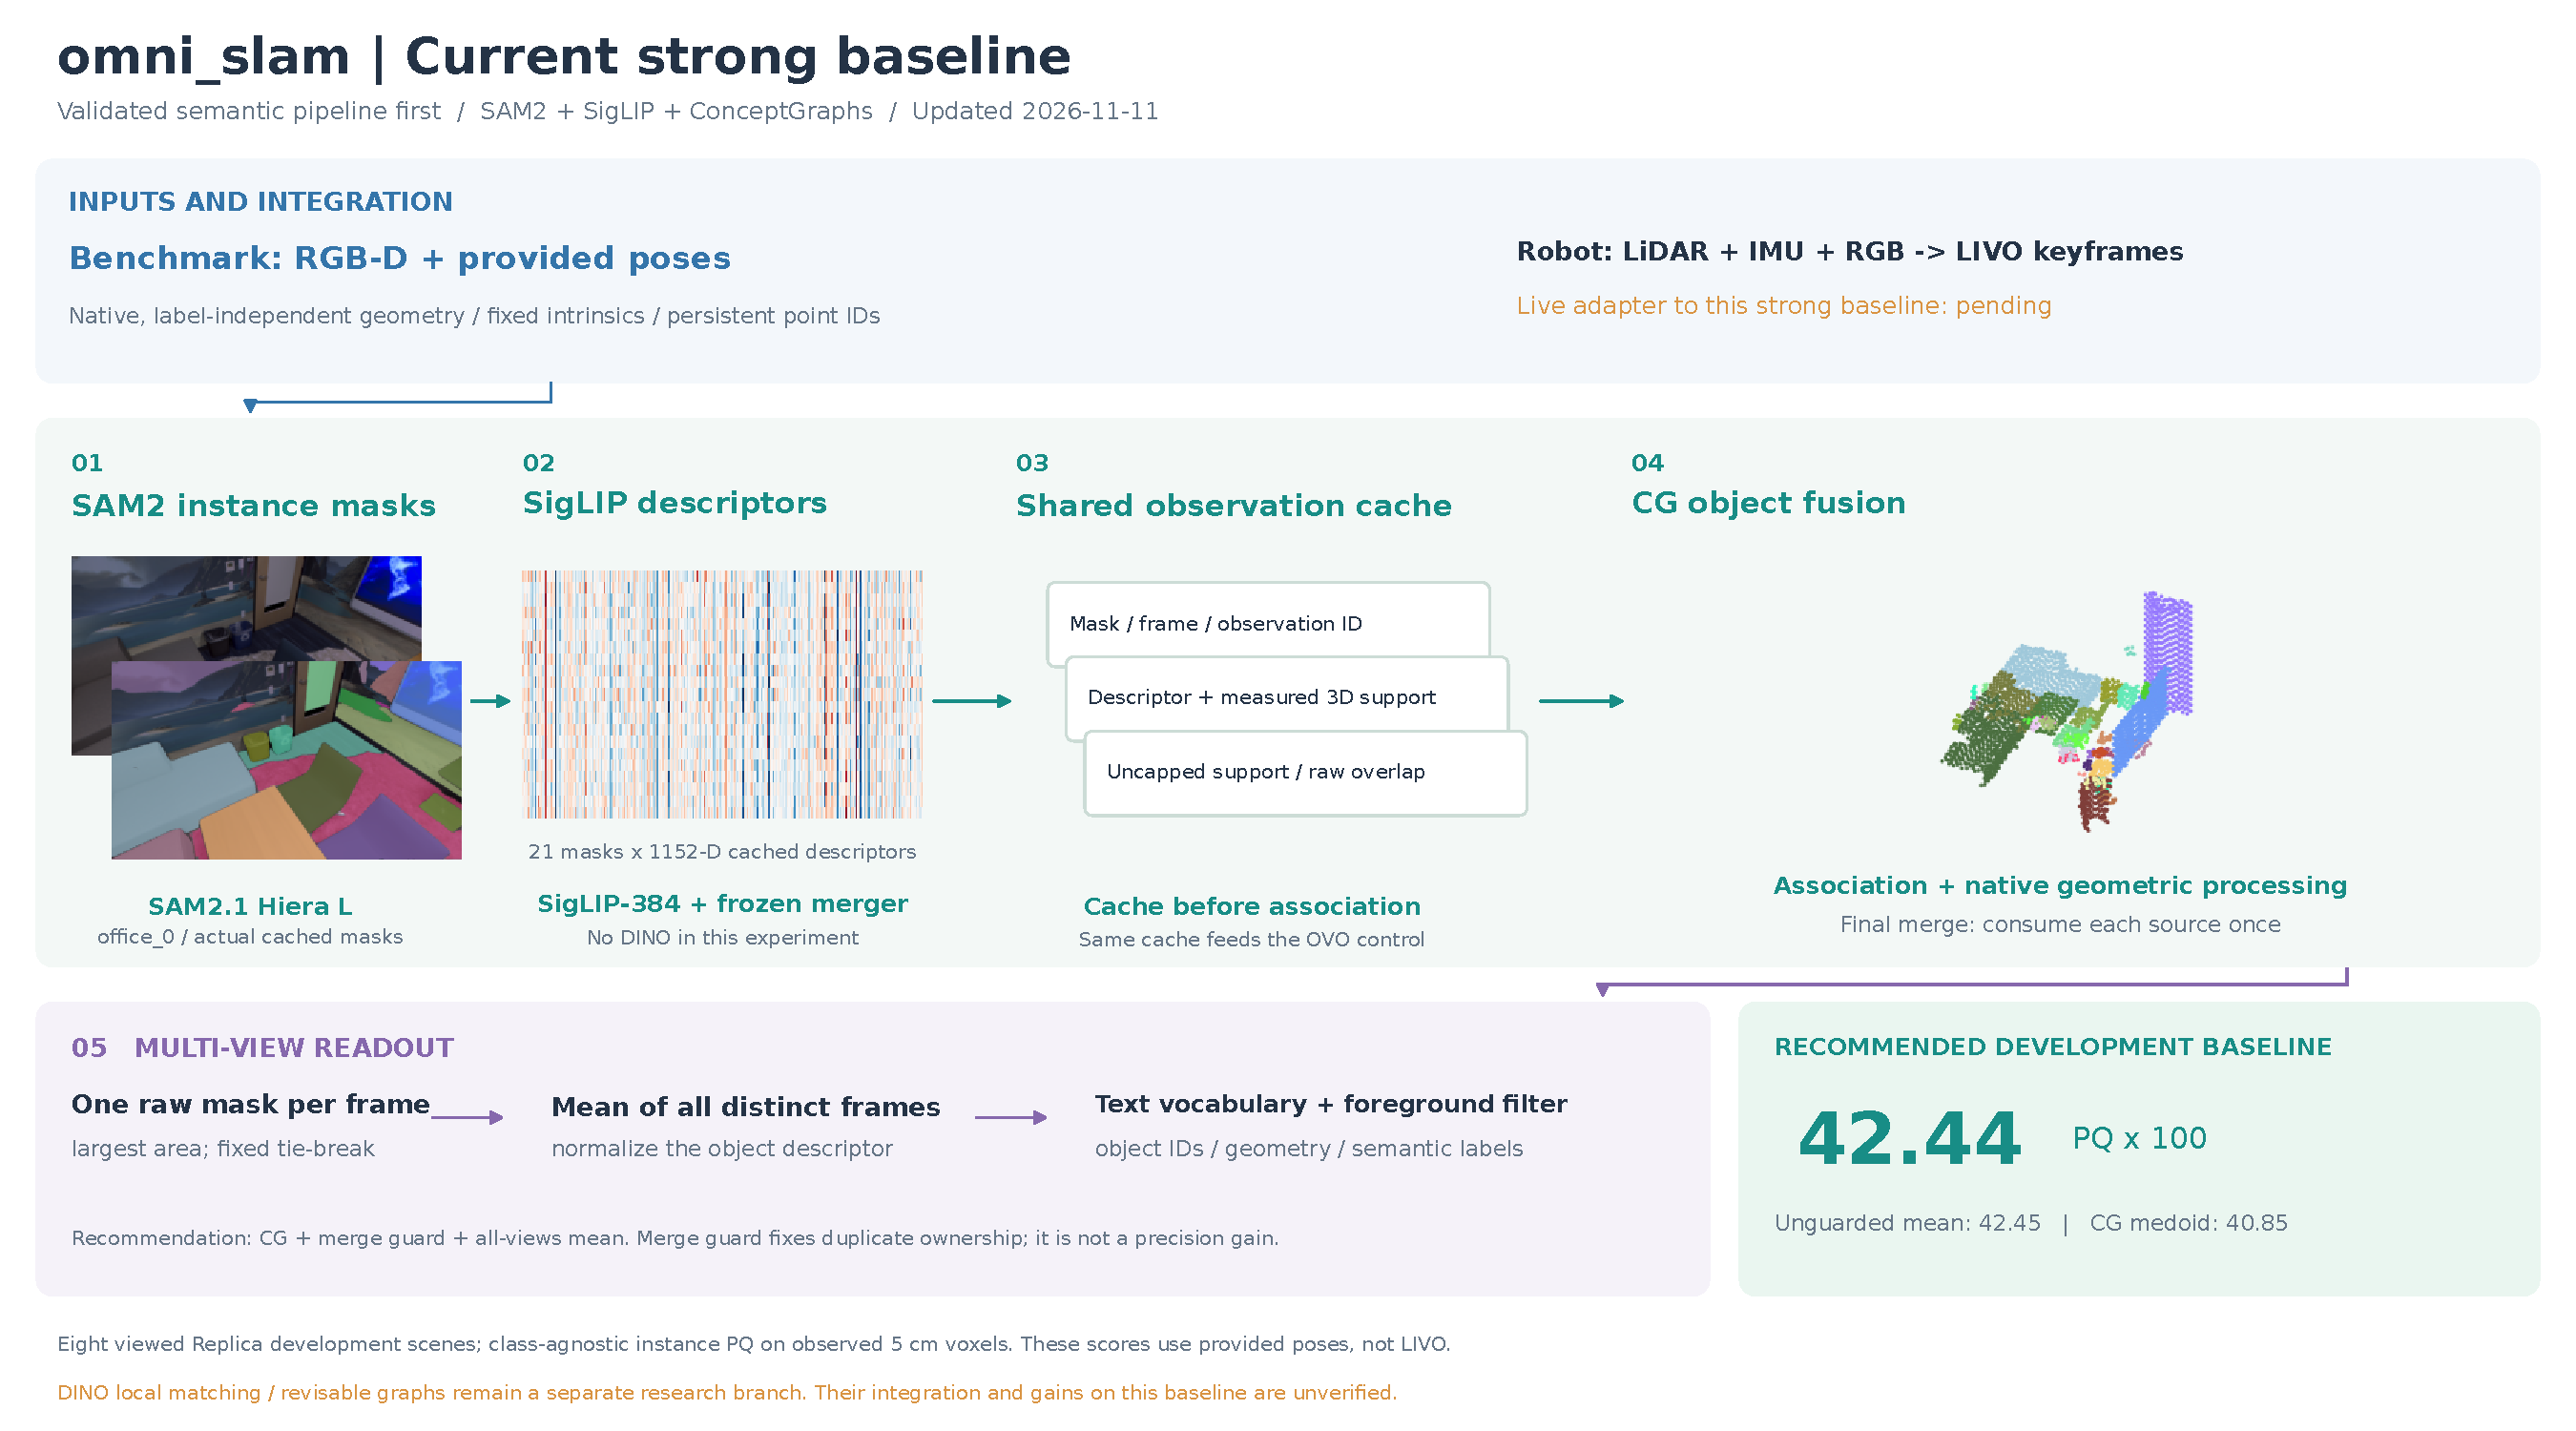
\includegraphics[width=\textwidth]{figures/history/omni_slam_current_baseline.pdf}
\captionof{figure}{Strong-baseline diagram from 11 November 2026. SAM2 and frozen SigLIP produce shared observations for ConceptGraphs-style fusion, a source-consumption guard, and a unique-frame mean semantic readout. The embedded title ``Current strong baseline'' refers to that dated revision. The 42.44 PQ value is from eight already-viewed Replica development scenes under its own observed 5\,cm domain; it is not current authorization performance.}
\end{center}
\subsection{What this diagram preserves}
The figure records the shared frontend, geometric fusion, and semantic readout before the later revision studies. Its robot adapter and DINO enhancement markers are design status from that revision. Current outdoor evaluation uses the separately documented SAM3-based branch; scores from these versions must not be pooled.

\clearpage
\section{Archived DINO--LIVO System Design}
\begin{center}
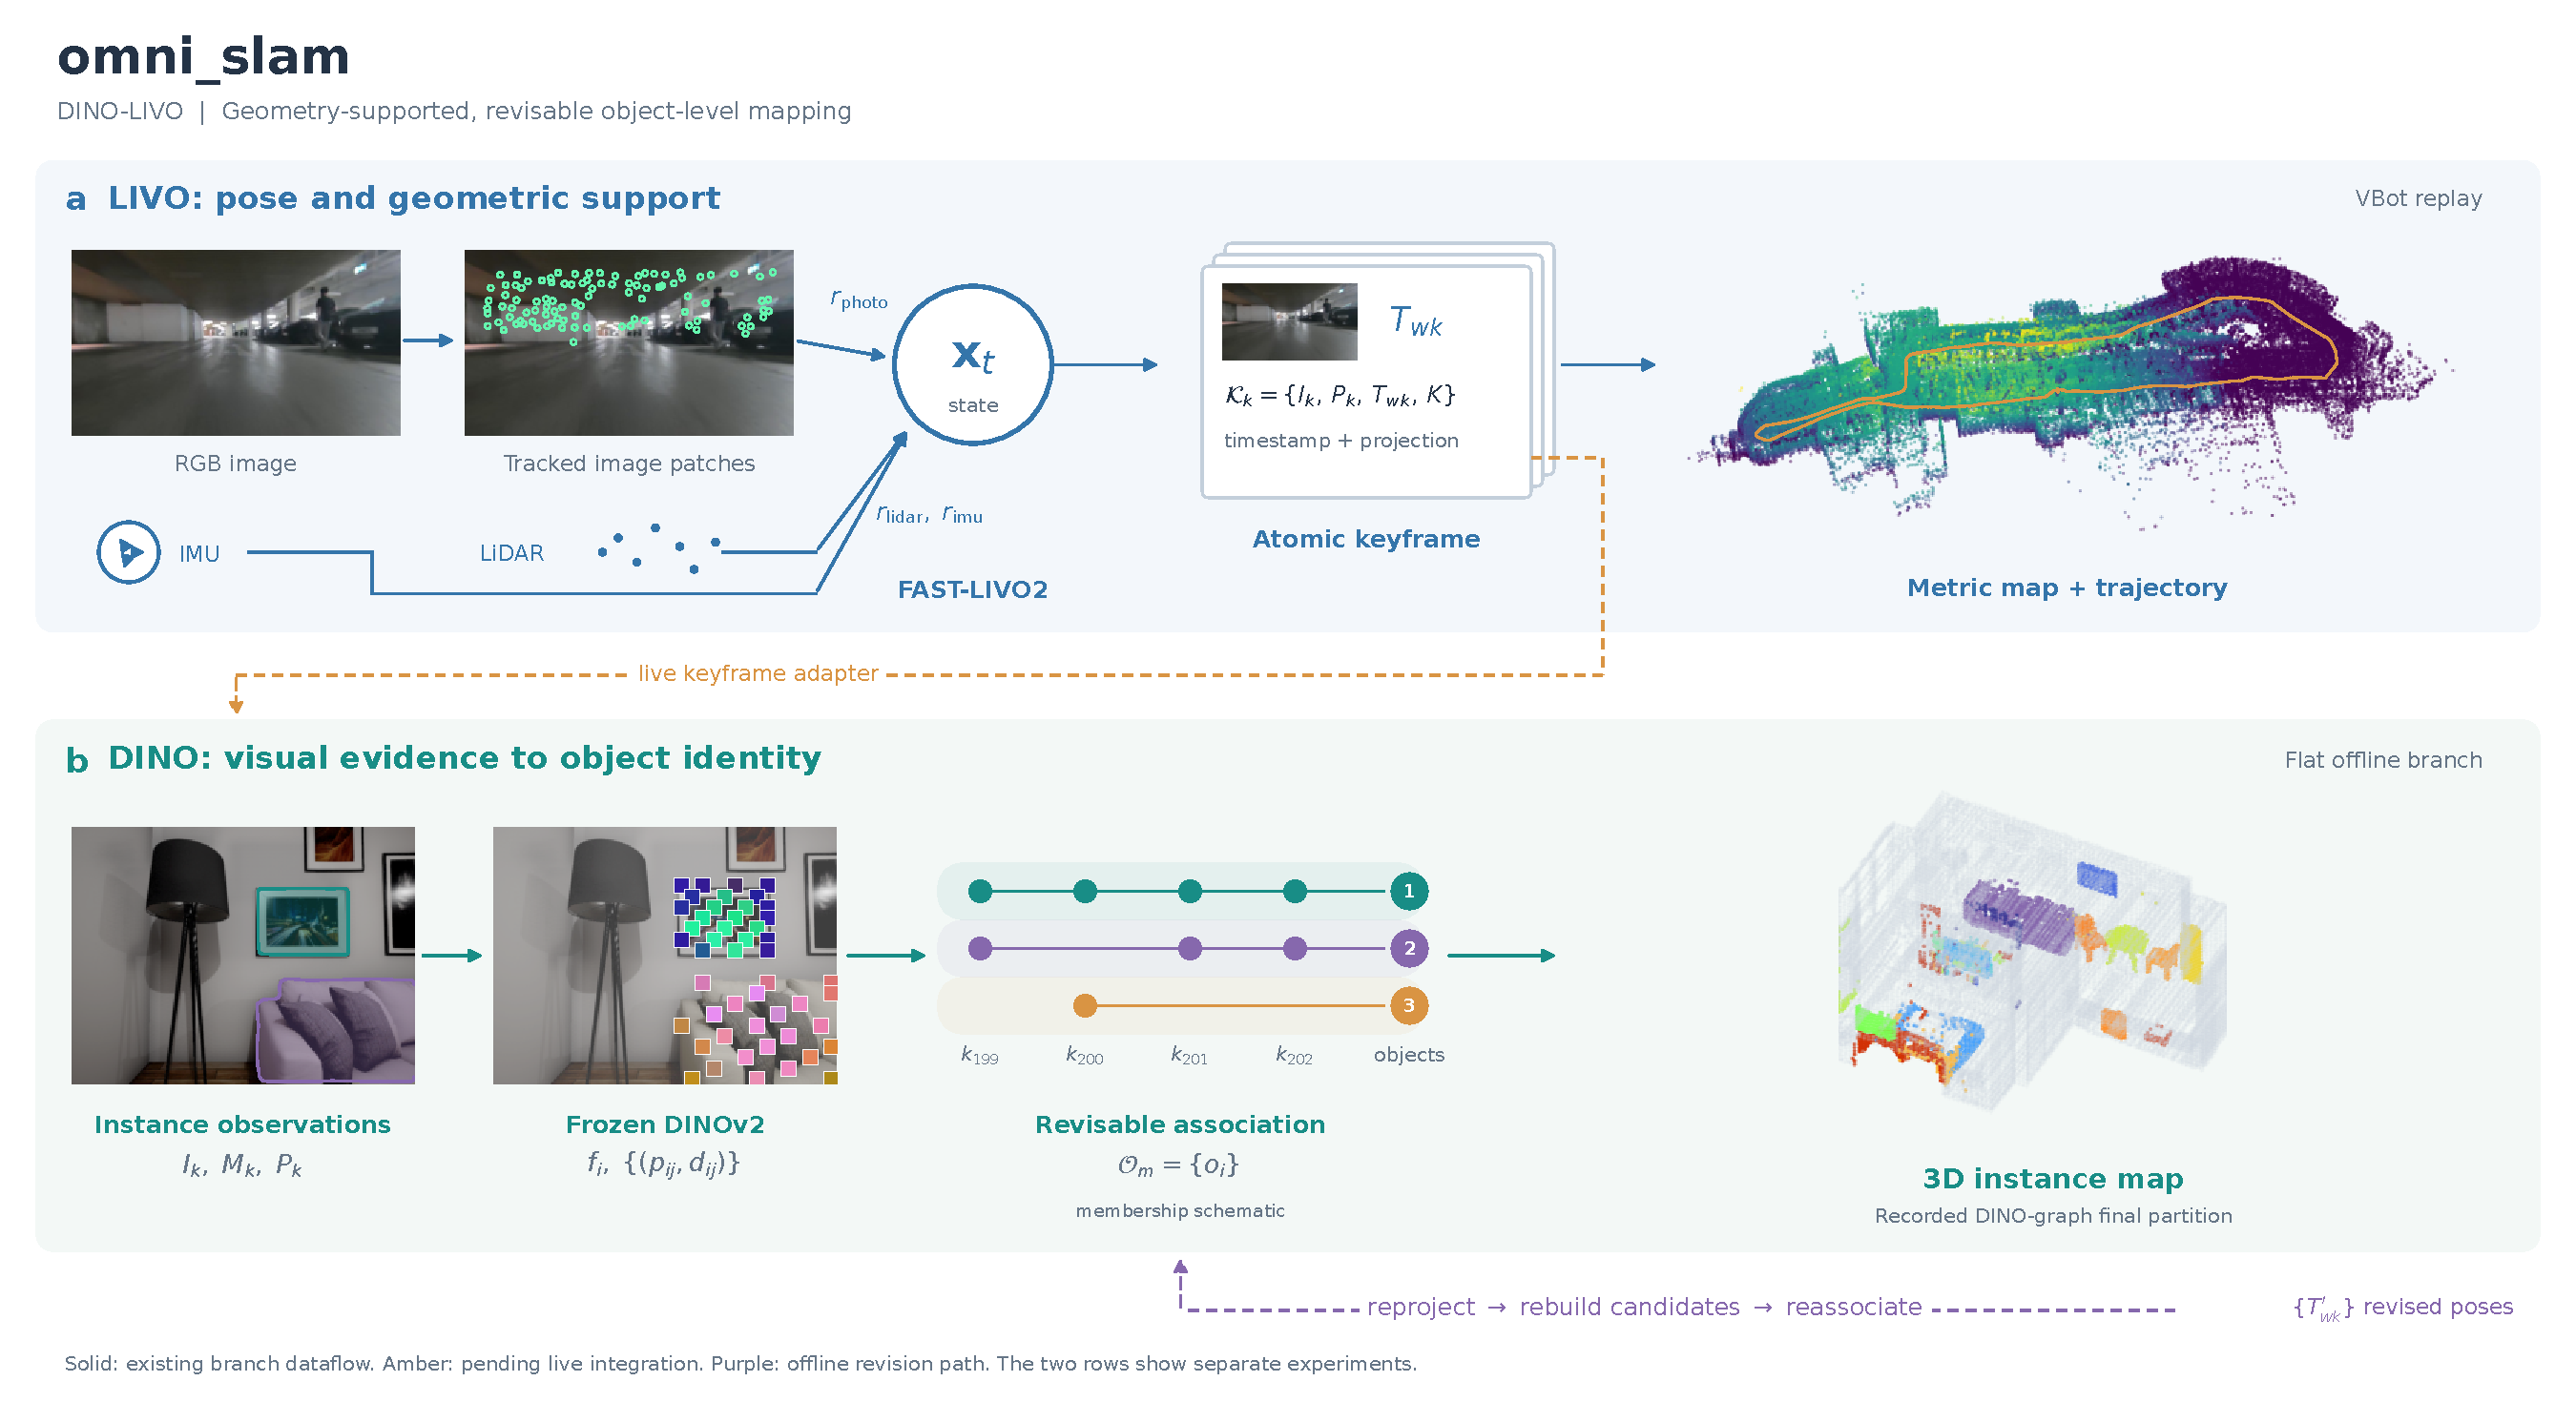
\includegraphics[width=\textwidth]{figures/history/dino_livo_system_architecture.pdf}
\captionof{figure}{DINO--LIVO design from 10 November 2026. The upper panel uses real VBot LIVO replay, while the lower panel uses a separate Flat offline DINO experiment. LIVO exports measured geometry and keyframes; frozen DINOv2 descriptors support an observation graph. The amber dashed connector denotes proposed live integration. This is not a jointly evaluated end-to-end system or the architecture used to obtain current outdoor AP.}
\end{center}
\subsection{Sensor and semantic interfaces}
The design retains the intended interface from image, LiDAR, and inertial processing to object observations and persistent identities. The two panels use different experiments and do not imply a shared trajectory or coordinate frame. DINOv2 feature extraction is distinct from Grounding DINO detection in the archived outdoor landmarks.

The current paper evaluates object-map revision with a frozen backbone. This archived design explains the broader project context; it does not imply that DINO tokens modify LIVO residuals or that a new association Transformer has been trained.

\clearpage
\section{Archived DINO Object-Graph Detail}
\begin{center}
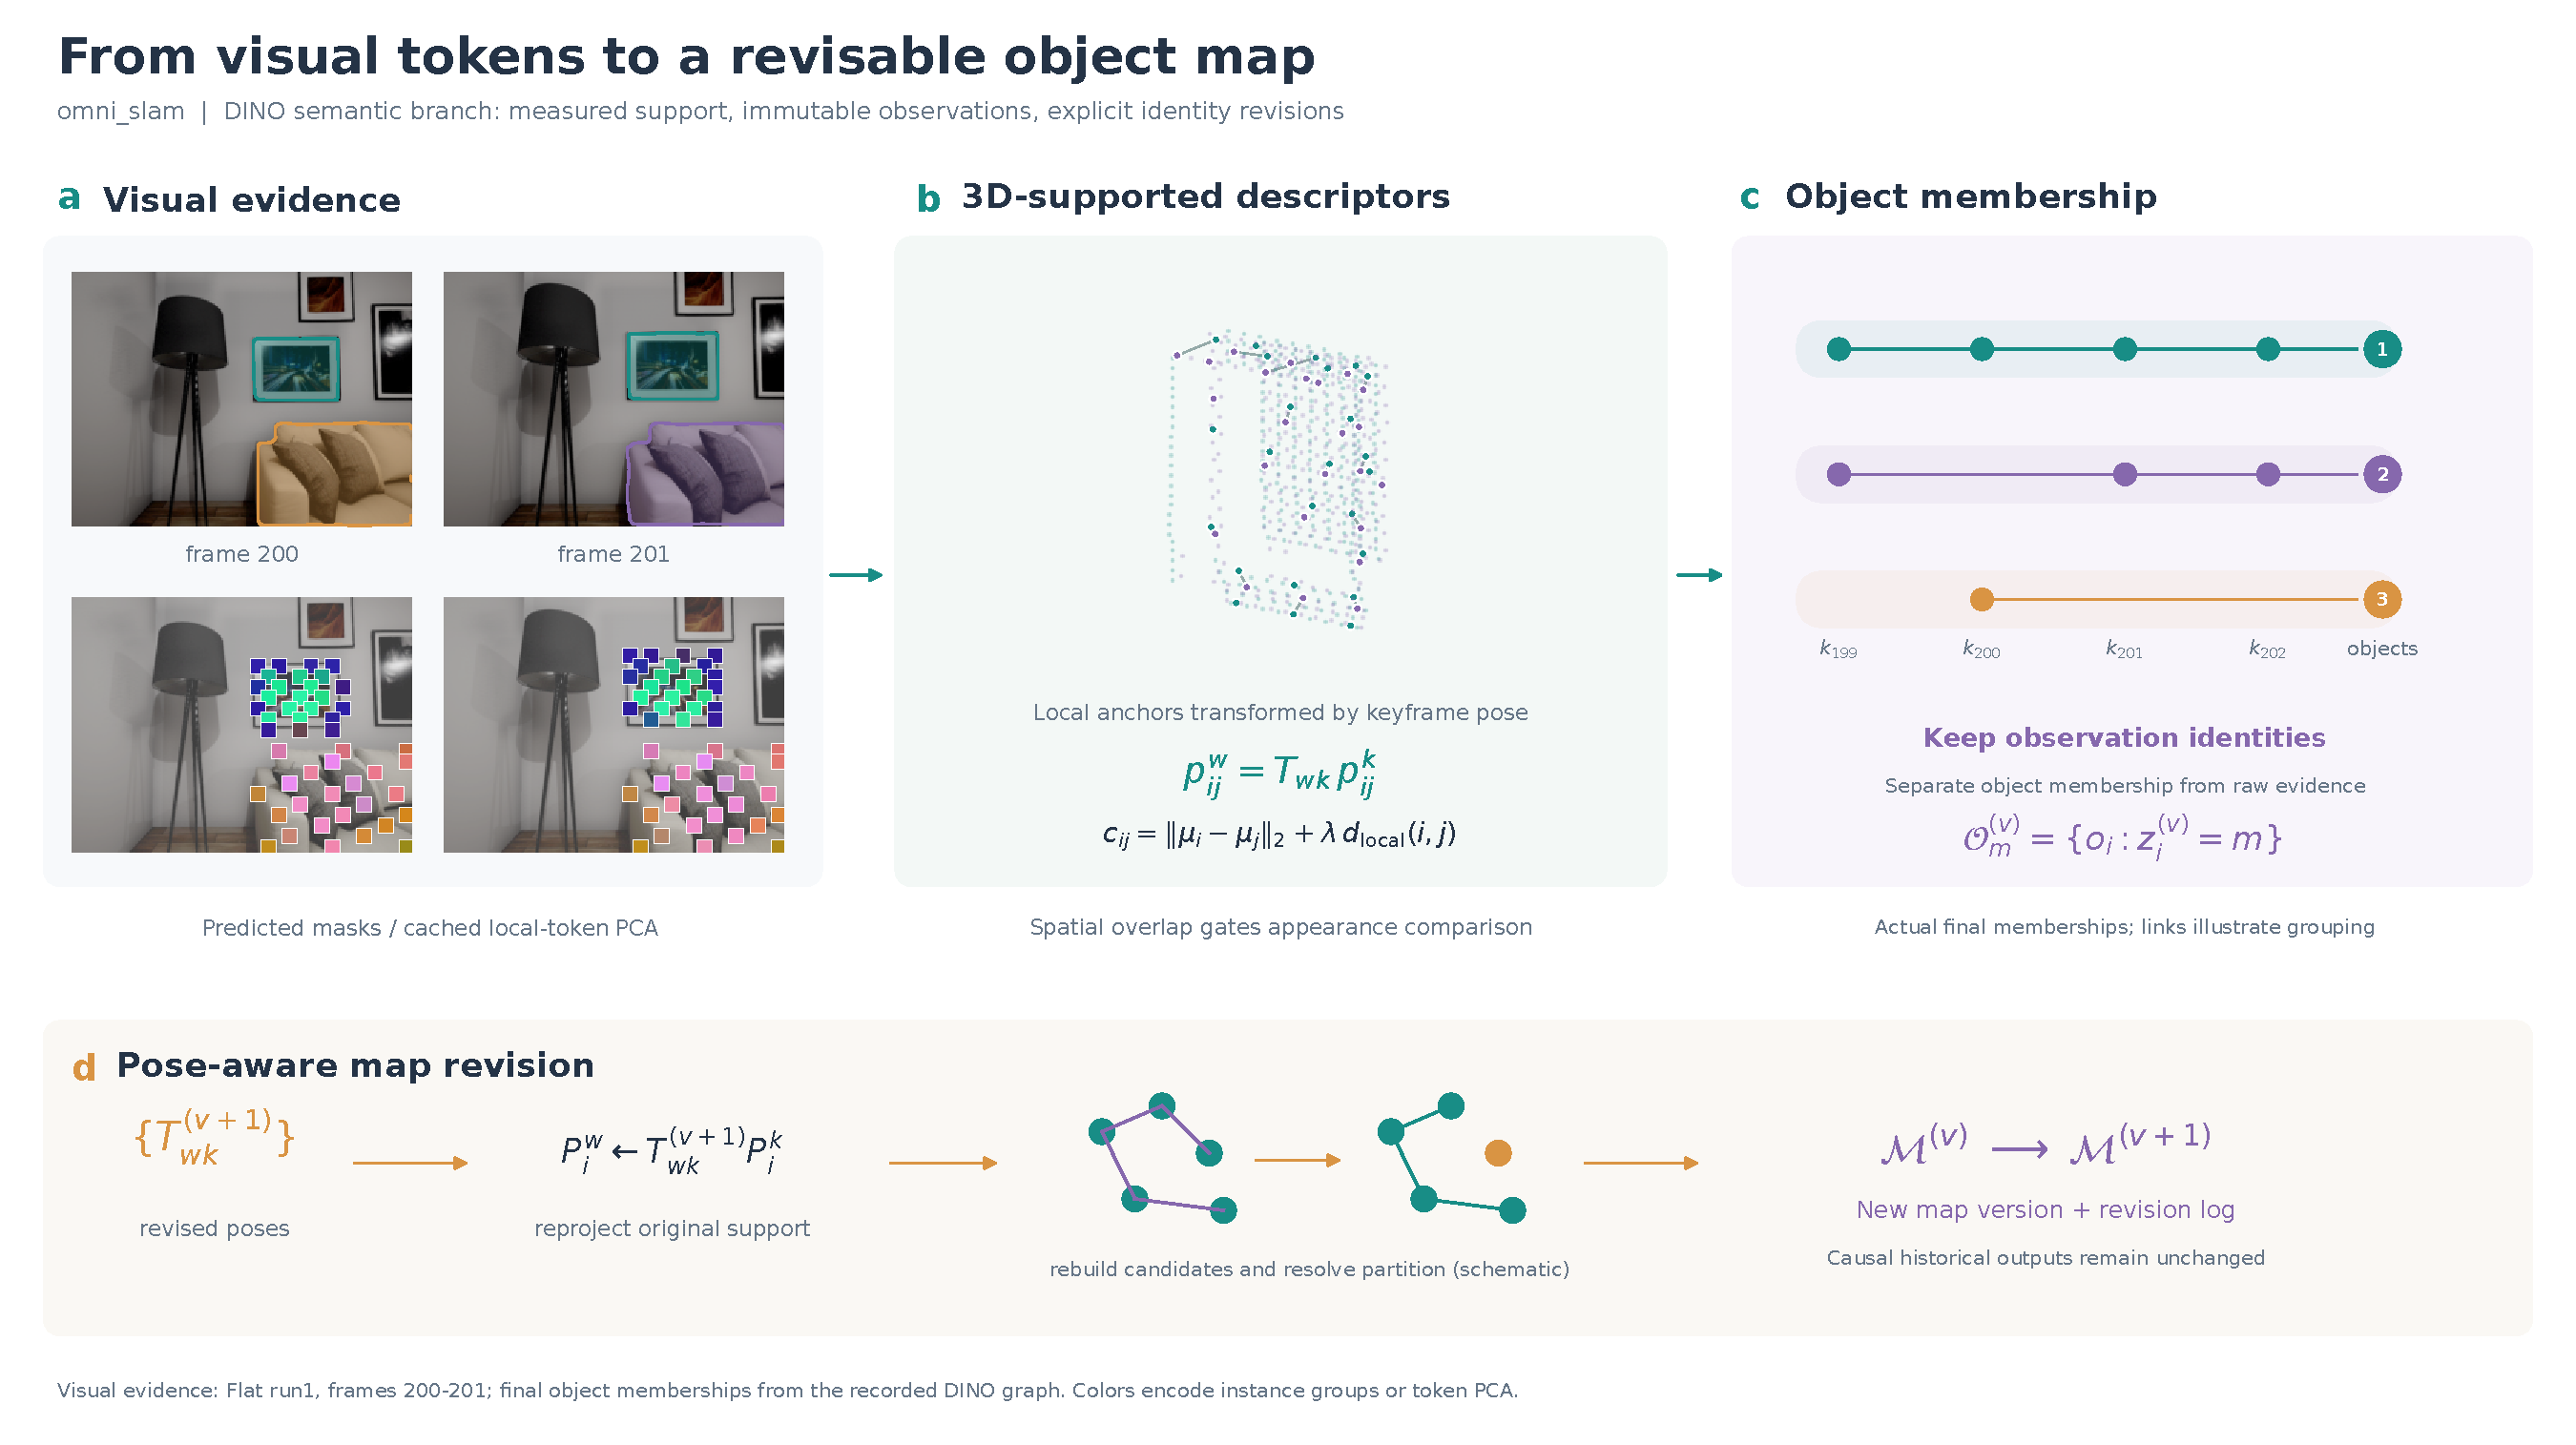
\includegraphics[width=\textwidth]{figures/history/dino_object_graph_detail.pdf}
\captionof{figure}{Geometry-supported DINO observations and map-revision design. Actual Flat run1 frames 200 and 201 supply masks and cached local descriptors, shown in one shared PCA basis. Measured depth anchors features in 3D; spatial support gates appearance comparison. Star links show recorded final memberships over frames 199--202, not original candidate edges. The pose-revision topology is schematic.}
\end{center}
\subsection{Interpretation of recorded memberships}
The displayed object numbers 1/2/3 correspond to original IDs 429/191/556. A sofa observation has different memberships across the selected frames; the original record is retained rather than presented as a repaired success. Feature colors are PCA visualizations, not semantic classes, attention weights, or matching confidence.

The diagram preserves an earlier candidate mechanism. It is neither an ablation of the current authorization rule nor evidence of stable DINO gains. The original input manifests are included with the three diagrams under \texttt{figures/history/}.

